\documentclass[12pt,oneside]{report}
\usepackage{setspace}\doublespacing
\usepackage{physics}
\usepackage{amssymb}
\usepackage{amsmath}
\usepackage{subcaption}
\usepackage{graphicx}
\usepackage{lipsum}
\usepackage{titlesec}
\usepackage{microtype}
\usepackage{appendix}
\usepackage[all]{nowidow}
\usepackage{bm}
\renewcommand{\vec}[1]{\text{\bfseries #1}}
\graphicspath{{images/}}
\input{spp.dat}
\pretolerance=5000
\tolerance=9000
\emergencystretch=0pt
\righthyphenmin=4
\lefthyphenmin=4
%\widowpenalty10000
%\clubpenalty10000
\renewcommand*\thesection{\arabic{chapter}.\arabic{section}}

\def\email#1{\gdef\@email{#1}}\email{}


\begin{document}
\pagenumbering{roman}

\title{
	\Large\uppercase\expandafter{Compressive sensing: Applications from 1-D to N-D
	}
}

\author{
	\large\rm\expandafter{
	Kenneth V. Domingo 
	}\\
	\large\textit{\expandafter{
		kdomingo@nip.upd.edu.ph
	}}\\
	\textsc{An Undergraduate Thesis Submitted to}\\
	\textsc{National Institute of Physics}\\
	\textsc{College of Science}\\
	\textsc{University of the Philippines} \\
	\textsc{Diliman, Quezon City}\\
	\vskip0.25in
	\rm In Partial Fulfillment of the Requirements\\
	\rm for the Degree of\\
	\rm\uppercase\expandafter{Bachelor of Science}
	\rm\uppercase{in}
	\rm\uppercase\expandafter{Applied Physics}\\
	\textsc\expandafter{April 2020}
}

\maketitle
\thispagestyle{titlestyle}

\chapter*{Acknowledgments}

\chapter*{Abstract}

\tableofcontents
\listoffigures
\listoftables

\cleardoublepage
\pagenumbering{arabic}

The recent trend of curiosity-driven human development has caused a surge in the amount of openly accessible data. More often than not, the inflow of information into digital systems happens much faster than the system can process the data. Moore's law implicitly sets a limit to how powerful and how quick our electronic systems can become (barring a significant breakthrough in the field of quantum computing), and the Nyquist-Shannon sampling theorem (NST) limits the range of frequencies a certain device can successfully recover. This study explores the use of compressed sensing (CS)---an emergent sampling theorem that allows recovery of signals from much fewer samples than required by the NST---as a viable sampling method for signals with an arbitrary number of dimensions, for applications such as compression, encryption, and enhancement. In this framework, the computational burden is shifted from the sampling device to the device performing reconstruction/decompression, and as such, there exist many ways to recover a signal from compressive measurements. The use of CS has been applied to simple audio signals containing pure tones \cite{Mathew2016,Andras2018} and speech \cite{Low2013,Low2018,Abrol2015}, images \cite{Mo2013,Zhou2016,Romero2016}, and videos \cite{Liu2014,Chen2014}. Common implementations of CS utilize analytical measurement bases such as the discrete cosine transform (DCT) basis, but recent studies \cite{Liu2013,Sharma2018,Eslahi2016} have shown that learned bases perform much better on more complex signals, i.e., those one would typically encounter in practical situations. The learning algorithms associated with these bases range from the classical iterative methods, such as matching pursuit (MP) and principal components analysis (PCA), to the more contemporary machine learning methods, most notably recurrent neural networks (RNN) and associative memory neural networks (AMNN). The novelty of this study is to provide a generalization of compressive sensing methods on signals of arbitrary dimensions.


\section{Related literature}
\label{sec:rrl}
In 2006, Cand\`{e}s, Romberg, Tao \cite{Candes2006}, and Donoho \cite{Donoho2006} kicked off the field of compressive sensing by answering the following question: ``With the recent breakthroughs in lossy compression technologies, we now know that most of the data we acquire can be thrown away with minimal perceptual loss. Why bother to acquire all the data when we can just directly measure the part that will not be thrown away?'' The methods in CS apply concepts from time-frequency uncertainty principles \cite{Donoho2001} and sparse representations \cite{Donoho2003}. CS can be viewed as a random but strategic undersampling method, where the sampling rate can be associated with a quasi-frequency which is significantly lower than the Nyquist rate, and the random samples usually follow Gaussian or uniform distribution. \cite{LinhTrung2008} demonstrated the use of deterministic chaos filters to acquire samples instead of random distributions. The chaotic behavior of the sampling function naturally led to exploring the use of CS as an encryption algorithm. This was used to achieve simultaneous compression and encryption in \cite{Mo2013}, and was extended in \cite{Zhou2016} to utilize higher-dimensional chaotic systems. Sampling using chaotic maps, such Gaussian-Logistic map, were applied to acoustic signals in \cite{Mathew2016}. In the methods above, sampling was performed in the real domain (i.e., time domain for audio, spatial domain for images), and the reconstruction was performed in the frequency domain. \cite{Andras2018} proposed a method to perform both sampling and reconstruction in the time domain using differential evolution.

Due to the relatively large size of video information, as a consequence of its high dimensionality, it is impractical to apply image CS techniques on an entire frame-by-frame basis. Correlations between adjacent frames are utilized instead, and can be obtained using dictionary learning \cite{Liu2013} or PCA \cite{Liu2014}. For the same reason, the application of CS to videos naturally led researchers to look towards machine learning methods \cite{Yao2019}. \cite{Iliadis2018} created the DR2-Net architecture which trains on image patches derived from grayscale videos to reduce dimensionality.

The application of CS for signal denoising was explored in \cite{Dabov2007}, and for recorded speech enhancement in \cite{Low2013}. Aside from the frequency domain, signals have been shown to be sparse in the modulation domain as well, which is a more appropriate representation for speech signals \cite{Low2018}, or other signals whose frequency contents may vary rapidly in time.


\section{Novelty}
\label{sec:novel}

\section{Compressive sensing}
\label{sec:cs}

Consider a signal which we wish to capture. This signal is real-valued and, depending on its dimensionality, can be represented as either a vector or a matrix. The acquisition of this signal can be modeled as a linear system, where the real signal values are transformed into values that can be understood by some sensing device or computer by applying a linear transformation by

\begin{equation}\label{eq:cesa}
    \vec{y} = \innerproduct{\vec{x}}{\vec{A}}
\end{equation}

\noindent where $\vec{A}$ is the transformation commonly known as a sensing matrix.

Consider a discrete time signal $\vec{x} \in \mathbb{R}^N$. Consider also an orthonormal basis $\bm\Psi \in \mathbb{R}^{N \times N}$ whose column vectors are expressed as $\bm\psi_i$. The signal $\vec{x}$ can be expressed as

\begin{equation}\label{eq:signal-transform}
	\vec{x} = \innerproduct{\bm\alpha}{\bm\Psi}
\end{equation}

\noindent where $\alpha_i$ are the coefficients of $\vec{x}$ in the $\bm\Psi$ domain. For practical signal processing applications, a sampled signal is usually of lower dimension than its original representation. We define the compressed vector $\vec{y} \in \mathbb{R}^M$, $M < N$ which is obtained by

\noindent where $\vec{A} \in \mathbb{R}^{M \times N}$ ($M \leq N$) is the sensing matrix. According to the NST, a periodic signal---which may be composed of a linear superposition of sinusoids with different parameters---has a characteristic bandwidth $f_B$, defined by its highest frequency component. The signal can be successfully reconstructed by a sampling device if the signal is sampled at a fixed rate with frequency $f_s$, which is at least twice $f_B$; that is $f_s \geq 2f_B$, where $2f_B$ is known as the Nyquist rate \cite{Shannon1949}. Under the NST, the original signal $\vec{x}$ in \eqref{eq:cesa} can be recovered by inversion, least squares approximation, or more commonly, sinc interpolation. More often than not, the inversion of \eqref{eq:cesa} is ill-posed because it is an underdetermined system. However, recovery is still possible provided that $\vec{x}$ is sparse or can be represented sparsely in some domain, and $\vec{A}$ satisfies one of the following properties \cite{Mazumdar2015}:
\begin{itemize}
	\item \textbf{Low mutual coherence}: The mutual coherence of a matrix $\vec{A}$ is defined as
	\begin{equation}
		\mu(\vec{A}) = \max_{i \neq j} \abs{\innerproduct{\vec{a}_i}{\vec{a}_j}}
	\end{equation}
	\item \textbf{Restricted isometry property} (RIP): Matrix $\vec{A}$ satisfies the RIP with sparsity parameter $k$ and restricted isometry constant $\delta$ if for all $k$-sparse vectors $\vec{x}$,
	\begin{equation}
		\qty(1 - \delta)\norm{\vec{x}}_2^2 \leq \norm{\vec{Ax}}_2^2 \leq \qty(1 - \delta)\norm{\vec{x}}_2^2
	\end{equation}
	\noindent The sparsity parameter $k$ entails that a vector has, at most, $k$ nonzero coefficients, in which case the vector is said to be $k$-sparse \cite{Candes2006}.
\end{itemize}

\noindent Once these have been satisfied, $\vec{x}$ can be recovered exactly from the compressive measurements $\vec{y}$ by solving the combinatorial minimization problem

\begin{equation}\label{eq:min-l0}
	\min \norm{\vec{x}}_0 \quad \textrm{subject to} \quad \vec{Ax = y}
\end{equation}

\noindent where $\norm{\vec{x}}_0$ denotes the $\ell_0$ pseudo-norm of $\vec{x}$, which extracts the number of nonzero coefficients. However, this problem is computationally intractable even for a small signal. A more tractable solution is to reduce this to a convex problem

\begin{equation}\label{eq:min-l1}
	\min \norm{\vec{x}}_1 \quad \textrm{subject to} \quad \vec{Ax = y}
\end{equation}

\noindent where $\norm{\vec{x}}_1 \equiv \sum_i \abs{x_i}$ denotes the $\ell_1$ norm of $\vec{x}$. For a sufficiently sparse signal, the solutions to \eqref{eq:min-l0} and \eqref{eq:min-l1} are identical \cite{Candes2006a}. A plethora of algorithms exist dedicated to solving \eqref{eq:min-l1}. The scope of this study utilizes the following algorithms used commonly in the literature:

\begin{itemize}
	\item \textbf{Least absolute shrinkage and selection operator} (LASSO): recasts the $\ell_1$ minimization problem as an $\ell_1$-regularized least squares problem:
	\begin{equation}
		\min_{\vec{x}} \frac{1}{2N} \norm{\vec{y} - \vec{Ax}}_2^2 + \alpha \norm{\vec{x}}_1
	\end{equation}
	where $\alpha$ is the regularization hyperparameter. Optimization is performed via coordinate descent \cite{scikit-learn}.
\end{itemize}
\chapter{Image compressive sensing}
\label{chap:image-cs}


One of the more intuitive applications of CS lies in spatial signals as it is easier to visualize. In this scheme, the process can be simplified either by flattening it to one dimension and processing it in its entirety, or maintaining its dimensionality and processing it by patches. The general workflow that arises from image CS is as follows:

\begin{enumerate}
	\item Define the compression ratio $m/n$, where $n$ is the signal size, and $m$ is the desired size of the compressed signal.
	\item Draw $m$ random indices from the signal without replacement and store this as a sample sequence $\bm\xi$.
	\item Extract the row vectors of the desired $n \times n$ sparsifying basis $\bm\Psi$ indexed by $\bm\xi$, and stack these to form the sensing matrix $\bm\Phi$ (i.e., $\bm\Phi = \bm\Psi_{\bm\xi}$)
	\item With the desired reconstruction algorithm, perform the optimization \eqref{eq:min-l1} to obtain the reconstructed signal $\bm\hat{\vec{x}}$.
\end{enumerate}

In the case of high-definition images (whose shortest side is at least 720 pixels), it is usually more practical and yields better results if the image is processed in patches.


\section{Test case: Sinusoidal pattern}
\label{sec:2dsin}
As mentioned in Chapter \ref{chap:theory}, the most commonly used sparse representation domain for images is the Fourier domain, referred to in some fields as $k$-space. In this space, signals are represented as a linear superposition of a finite number of sinusoidal patterns. In Fig. \ref{fig:2dsin}, $64 \times 64$ pixel sinusoidal patterns are generated, corresponding to sine waves traveling horizontally, vertically, and diagonally, as well as an egg tray pattern. In each case, all frequency components are 4 Hz. Figure \ref{fig:2dsin-masked} visualizes the compressed image when a random sample of 5\% is taken from the signal. The actual compressed signal that is seen by the reconstruction algorithm is a one-dimensional sequence containing only the information from the points being sampled. Orthogonal matching pursuit (OMP) was used for reconstruction, which is a greedy algorithm that finds the combination of basis vectors which best represents the signal (similar to matching pursuit), but in addition, the residual at each iteration is recomputed using an orthogonal projection on the set of previously selected basis vectors \cite{Mallat1993}. Its objective function is

\begin{equation}\label{eq:omp}
	\arg\min_{\vec{x}} \norm{\vec{y} - \bm\Phi \vec{x}}_2^2 \quad \textrm{subject to} \quad \norm{\vec{x}}_0 \leq \gamma
\end{equation}

\noindent where $\gamma$ is a hyperparameter which controls the maximum allowable number of non-zero coefficients. The Scikit-learn implementation sets this value to 10\% of the number of samples by default \cite{scikit-learn}. Evaluation of the mean-squared error (MSE) for the pure horizontal and pure vertical sine waves, as well as the egg tray pattern yields a value that is practically negligible ($\approx 10^{-31}$); the reconstruction is exact. On the other hand, the reconstructed diagonal sine wave yields an MSE of $10^{-3}$---still quite small, but mild distortion can be observed at the image boundaries. This is due to the fact that the information at hand is finite, and so is the window size which, in this case, is the same size as the signal itself.

\begin{figure}[tb]
	\centering
	\begin{subfigure}{\textwidth}
		\centering
		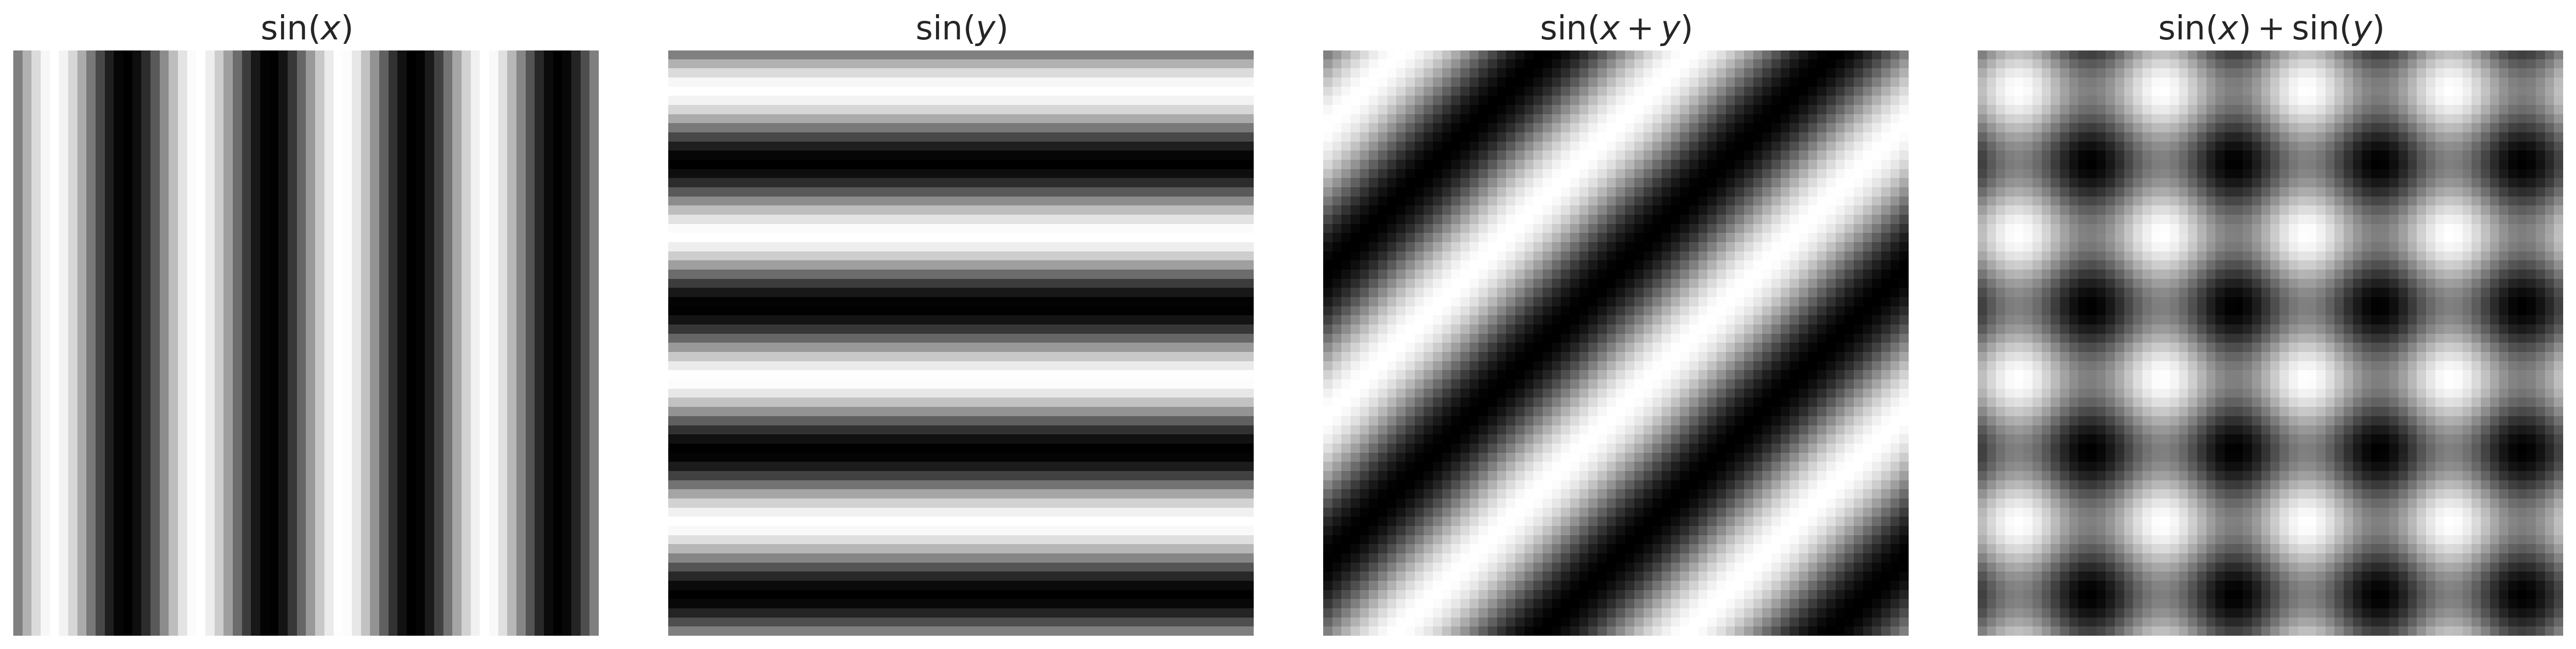
\includegraphics[width=\textwidth]{2dsin.png}
		\caption{Test 2D sinusoid patterns.}
		\label{fig:2dsin}
	\end{subfigure}
	\begin{subfigure}{\textwidth}
		\centering
		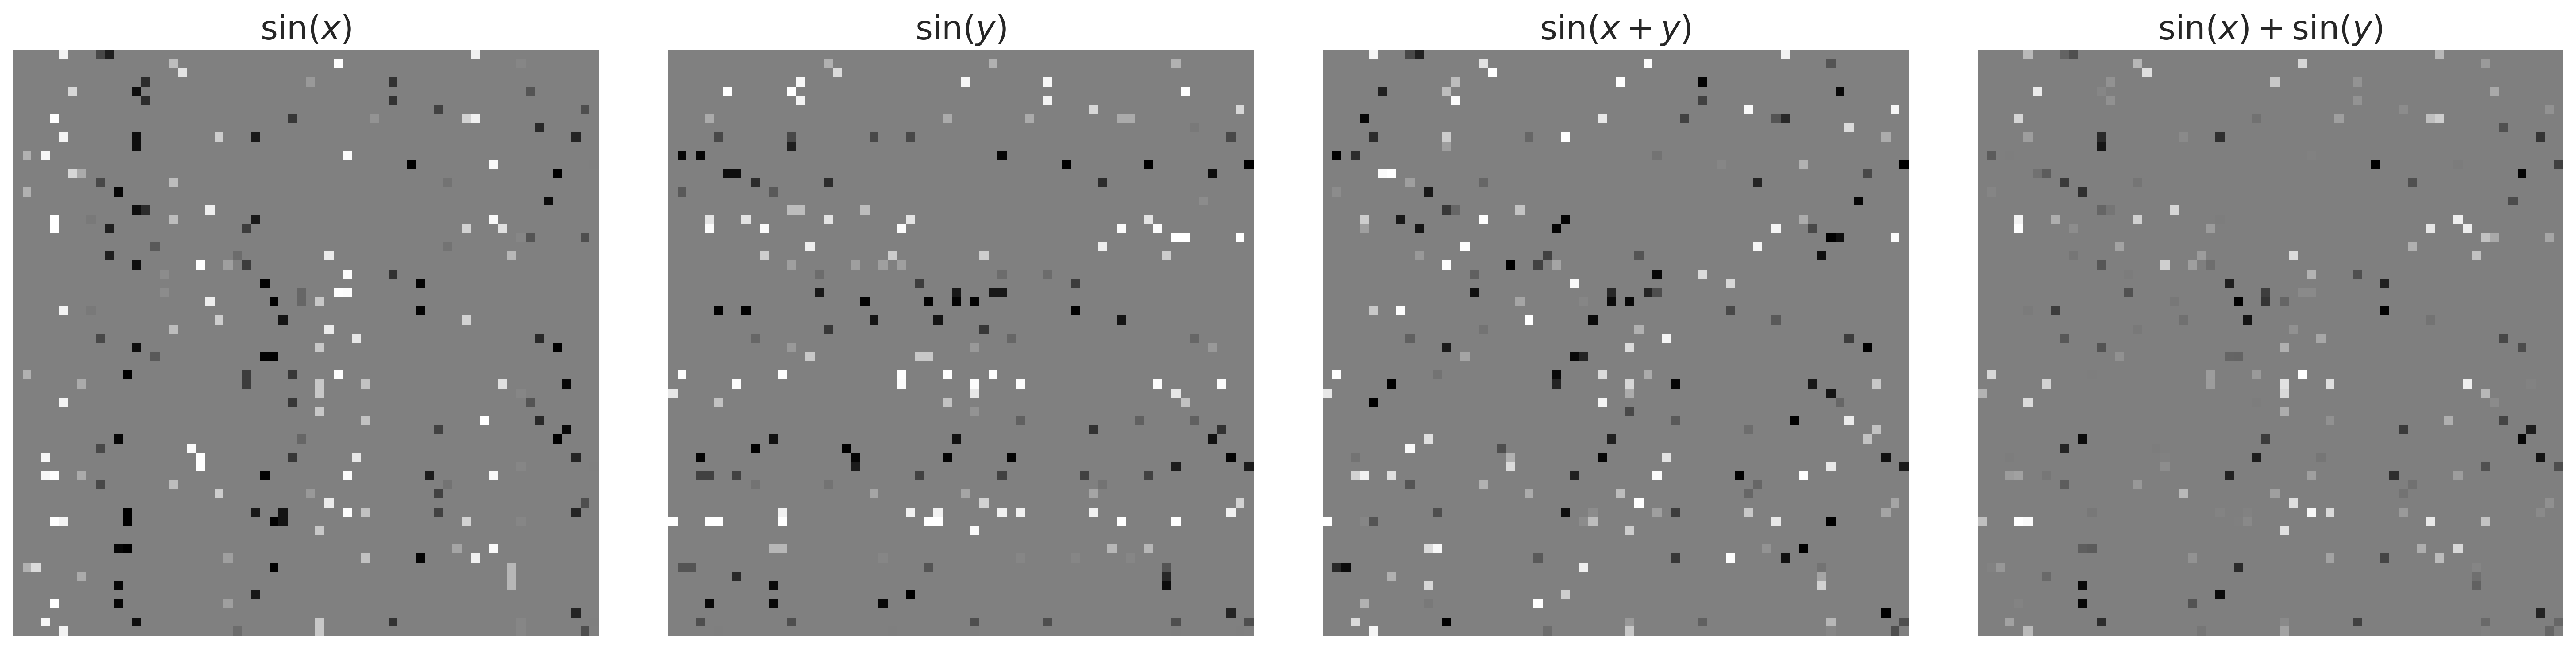
\includegraphics[width=\textwidth]{2dsin-masked.png}
		\caption{Visualization of sinusoid patterns with compression ratio of 5\%.}
		\label{fig:2dsin-masked}
	\end{subfigure}
	\begin{subfigure}{\textwidth}
		\centering
		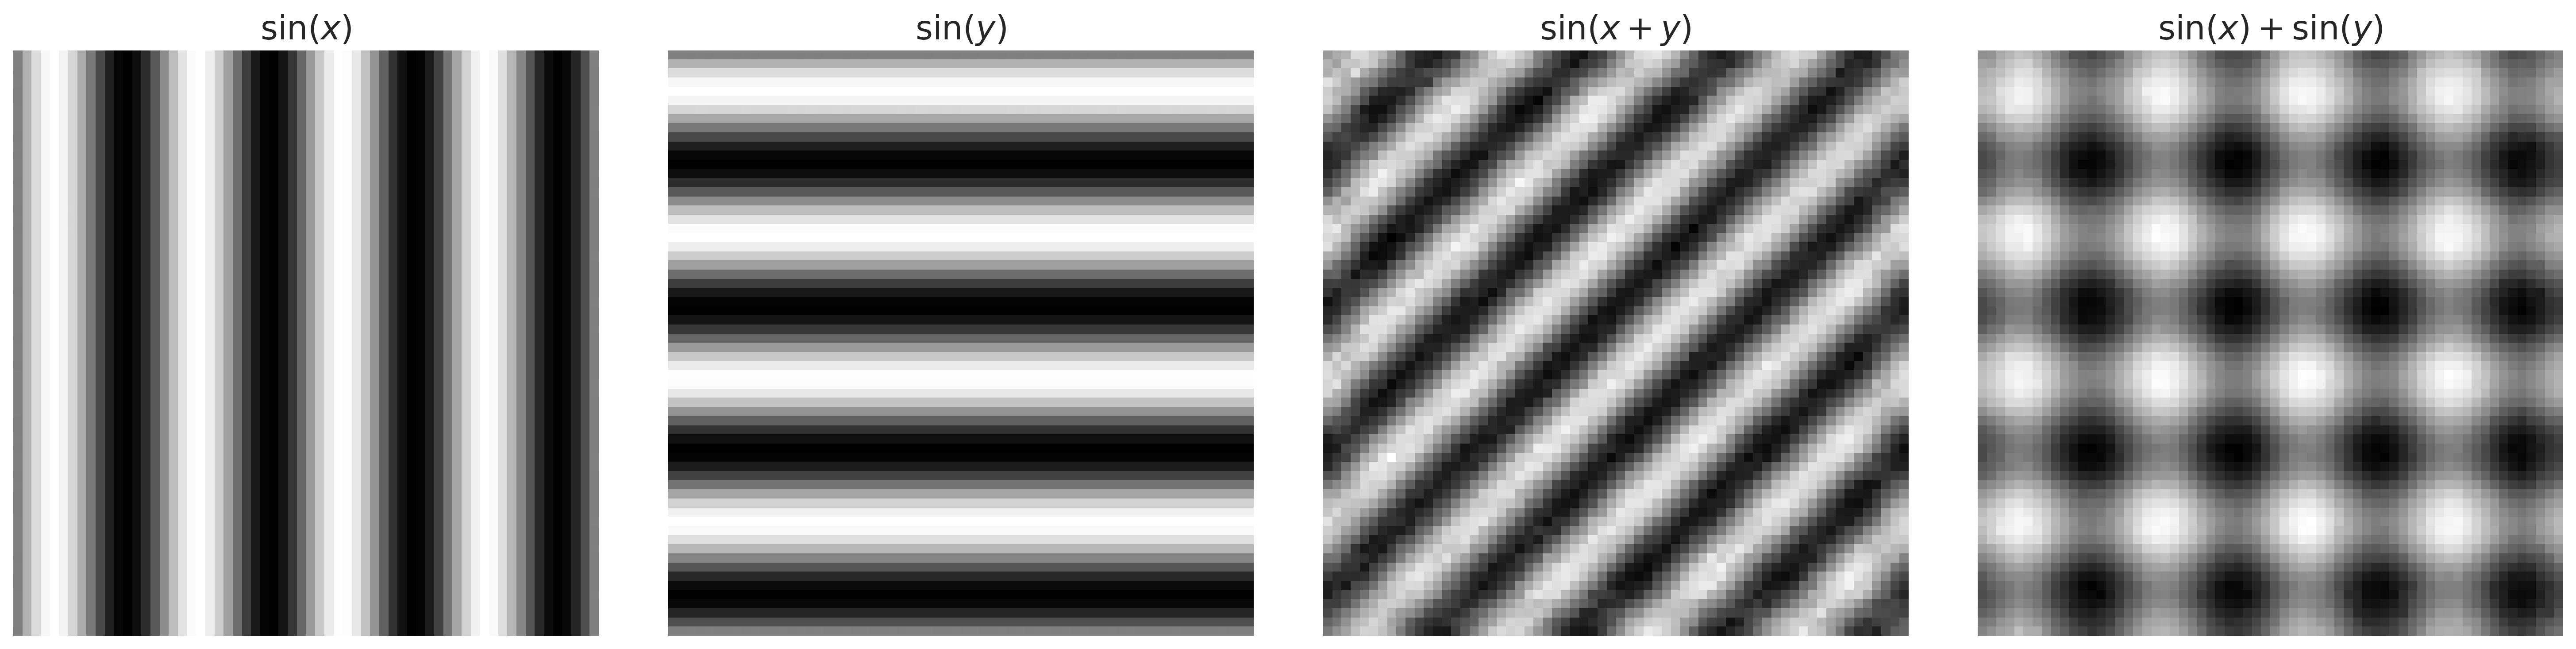
\includegraphics[width=\textwidth]{2dsin-recovered.png}
		\caption{Reconstruction from 5\% of samples.}
		\label{fig:2dsin-recovered}
	\end{subfigure}
	\caption{Test $64 \times 64$ pixel 2D sinusoid patterns corresponding to vertical sinusoids, horizontal sinusoids, diagonal sinusoids, and egg tray pattern. All frequency components are 4 Hz.}
	\label{fig:test-2dsin}
\end{figure}


\section{Image with multiple sinusoids}
\label{sec:2dmultisin}
For this section, the image used is M.C. Escher's \textit{Relativity}, an example of a more complex image but consisting of dominant sinusoidal patterns that are made apparent when you zoom in. The original image has dimensions of $1600 \times 981$ pixels, for a total of 1,569,600 pixels. Following the procedure with the previous section, this would require the construction of a 1,569,600 $\times$ 1,569,600 sparsifying matrix containing $\approx 2 \times 10^{12}$ entries. Assuming that the matrix would be stored as 32-bit floating point numbers, this process alone would take up $\approx 8$ GB of memory, and it would be highly impractical to process similarly-sized images as a whole. The workaround is to split it into smaller, manageable patches. For this image in particular, it was first resized to $1600 \times 976$ pixels so that it could be equally divided into a grid of $16 \times 16$, each with a dimension of $100 \times 61$ pixels. After compressively sampling each patch at 40\% compression ratio, reconstruction was performed using the Embedded Conic Solver (ECOS) of the Convex Optimization Python library (CVXPY), which recasts \eqref{eq:min-l1} as a convex problem and directly minimizes the $\ell_1$ norm \cite{ecos,cvxpy,cvxpy_rewriting} and thus, is significantly slower compared to OMP. After stitching all patches at the end, the reconstructed image is shown in Fig. \ref{fig:relativity-recovered}. Selected patches with the aforementioned dominant patterns are shown with their reconstructed counterparts in Fig. \ref{fig:relativity-dominant-slices}, corresponding to patches dominated by horizontal sinusoids, vertical sinusoids, diagonal sinusoids, multiple sinusoids, and patches with no dominant pattern. We can observe that at this compression rate, the patches with a single apparent sinusoidal pattern (Figs. \ref{fig:relativity-vert40}-\ref{fig:relativity-diag40}) are successfully recovered, with some noise present especially for the patch with a dominant diagonal pattern (similar to the previous section). The patch with multiple sinusoid patterns (Fig. \ref{fig:relativity-mult40}), although still recognizable, is laden with a lot of noise. Lastly, the patch with no apparent pattern (Fig. \ref{fig:relativity-high40}) is barely recognizable, except for the portions where a dominant sinusoidal pattern is partially present in the frame.

From this, the following information can be gleaned. First, reconstruction performs better on smaller patches, and when the patch in question contains as few frequency components as possible (such is the case with the patches with only one dominant pattern). Second, the patch with no dominant pattern---upon closer visual inspection---can be classified as being successfully recovered; however, the reconstruction noise is almost at the same level as the signal itself, which makes them indistinguishable. This can be attributed to the fact that the patches with no apparent dominant pattern are actually composed of a superposition of sinusoids residing primarily in the high-frequency region of $k$-space. Since the sampling points are uniformly distributed throughout the spatial domain, so are they in the frequency domain. Thus, the information in the high-frequency region is not sufficiently captured, and a higher compression ratio is required to be able to better recover these high-frequency regions. Another solution would be, as mentioned earlier, to make the patches smaller so that lesser frequencies are captured in one patch.

\begin{figure}[htb]
	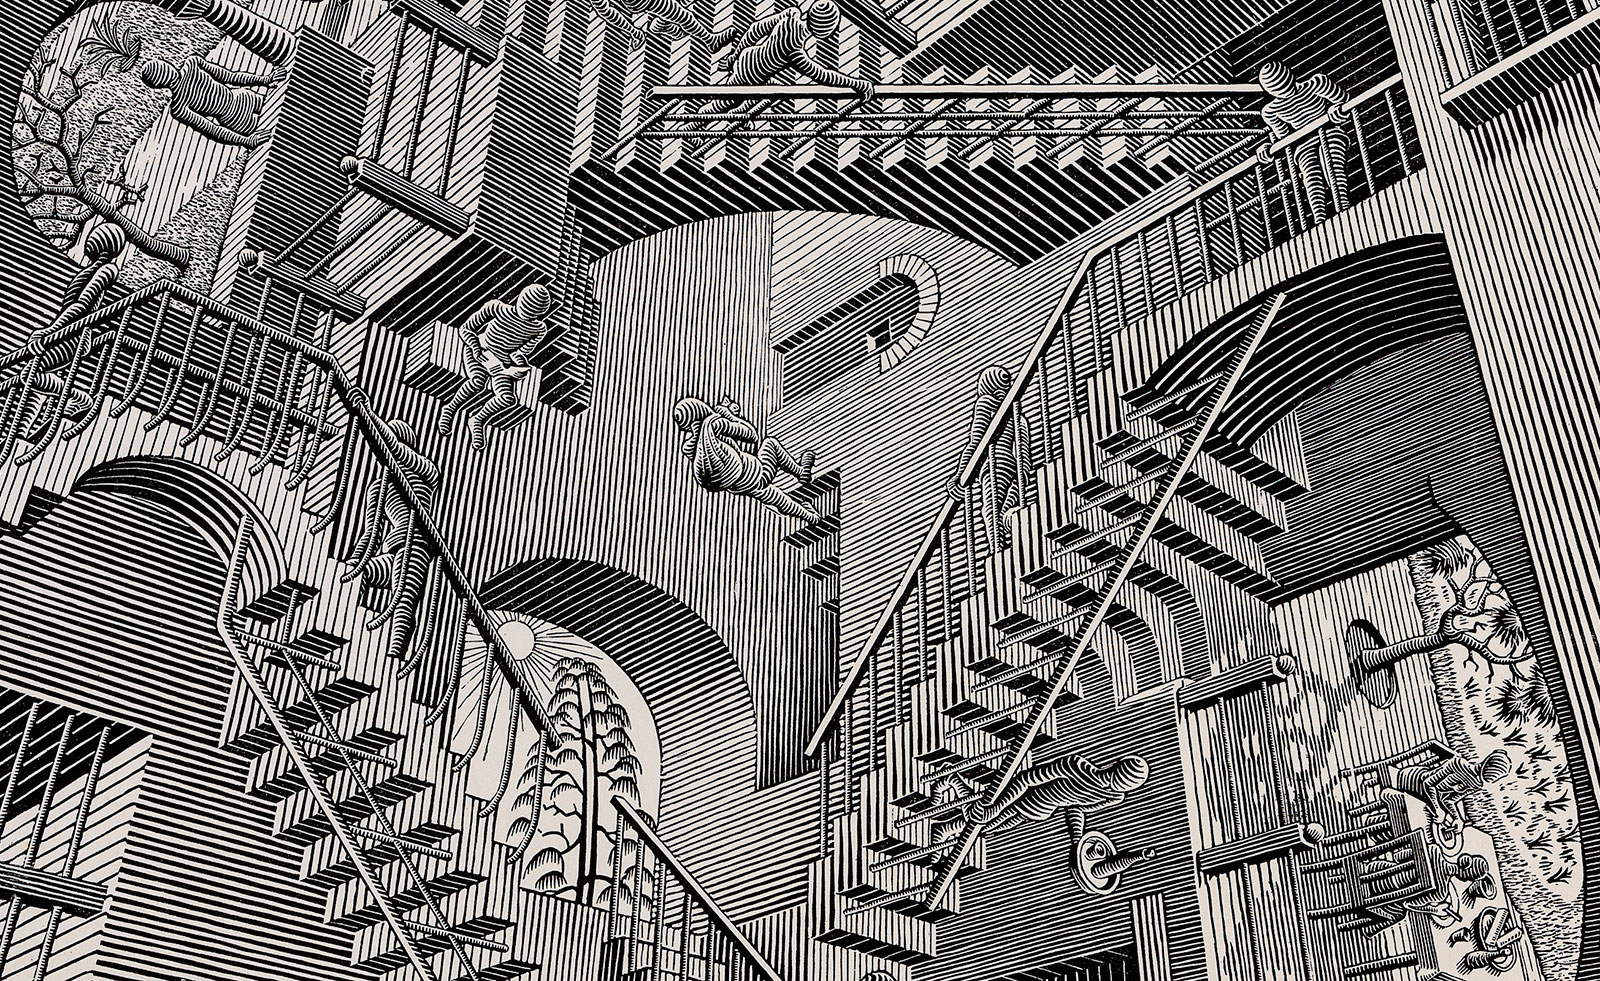
\includegraphics[width=\textwidth]{relativity.jpg}
	\caption{\textit{Relativity} by M.C. Escher, a complex image consisting of various sinusoidal patterns.}
	\label{fig:relativity}
\end{figure}

\begin{figure}[htb]
	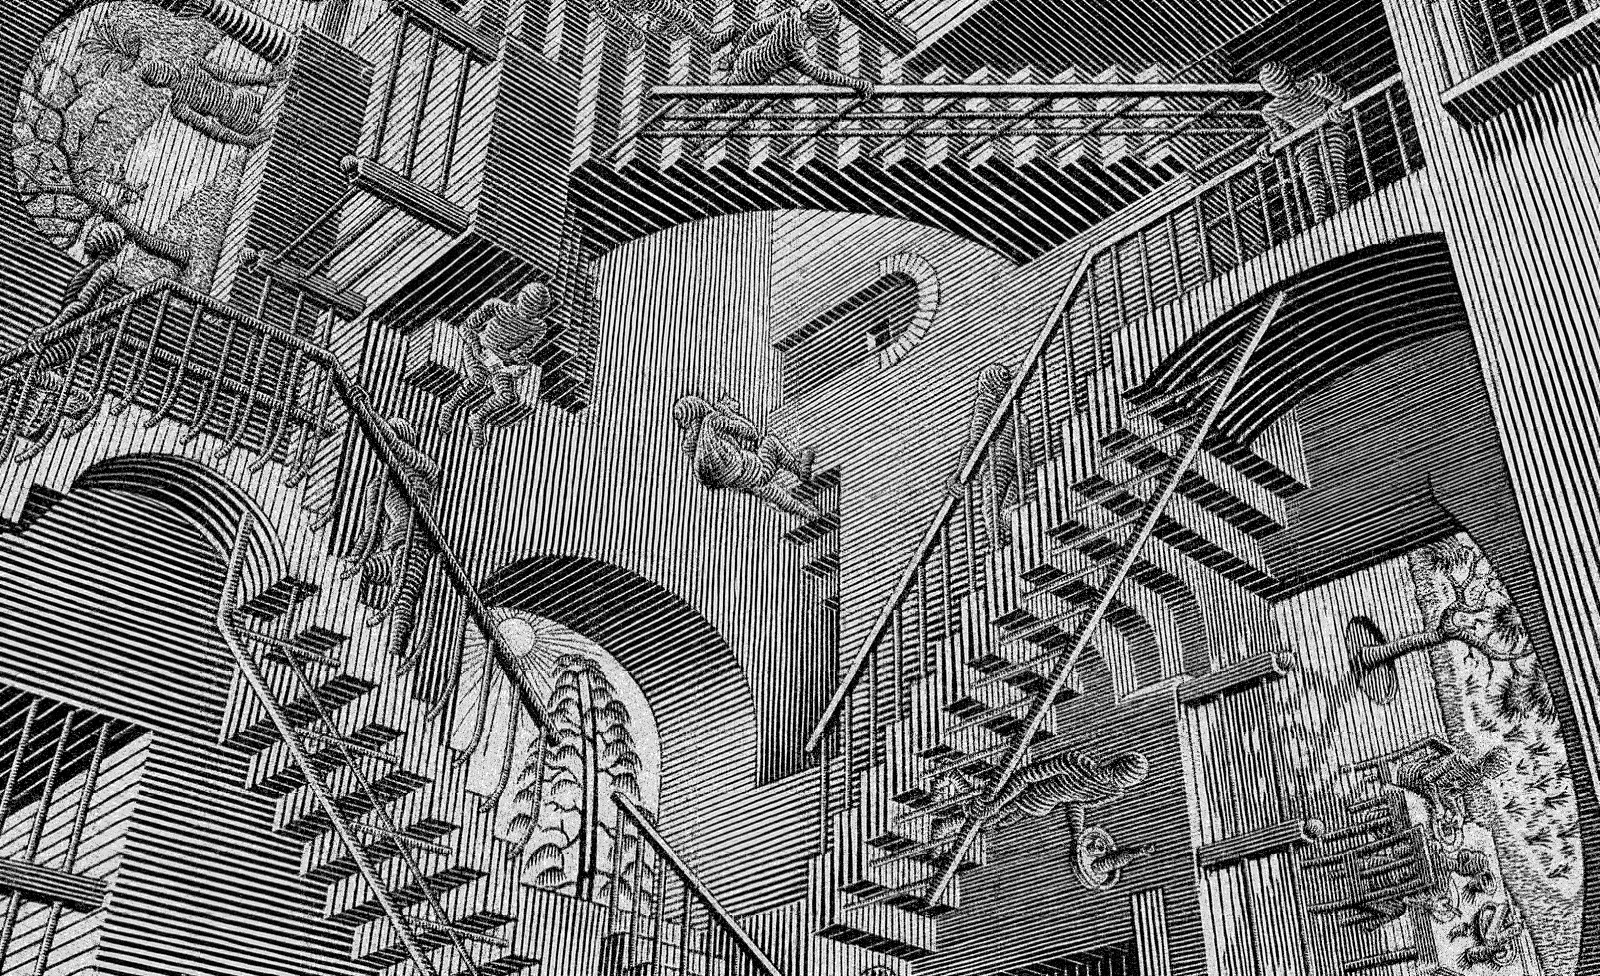
\includegraphics[width=\textwidth]{relativity-recovered.png}
	\caption{Reconstructed \textit{Relativity} from 50\% of samples from each patch.}
	\label{fig:relativity-recovered}
\end{figure}

\begin{figure}[htb]
	\centering
	\begin{subfigure}{\textwidth}
		\centering
		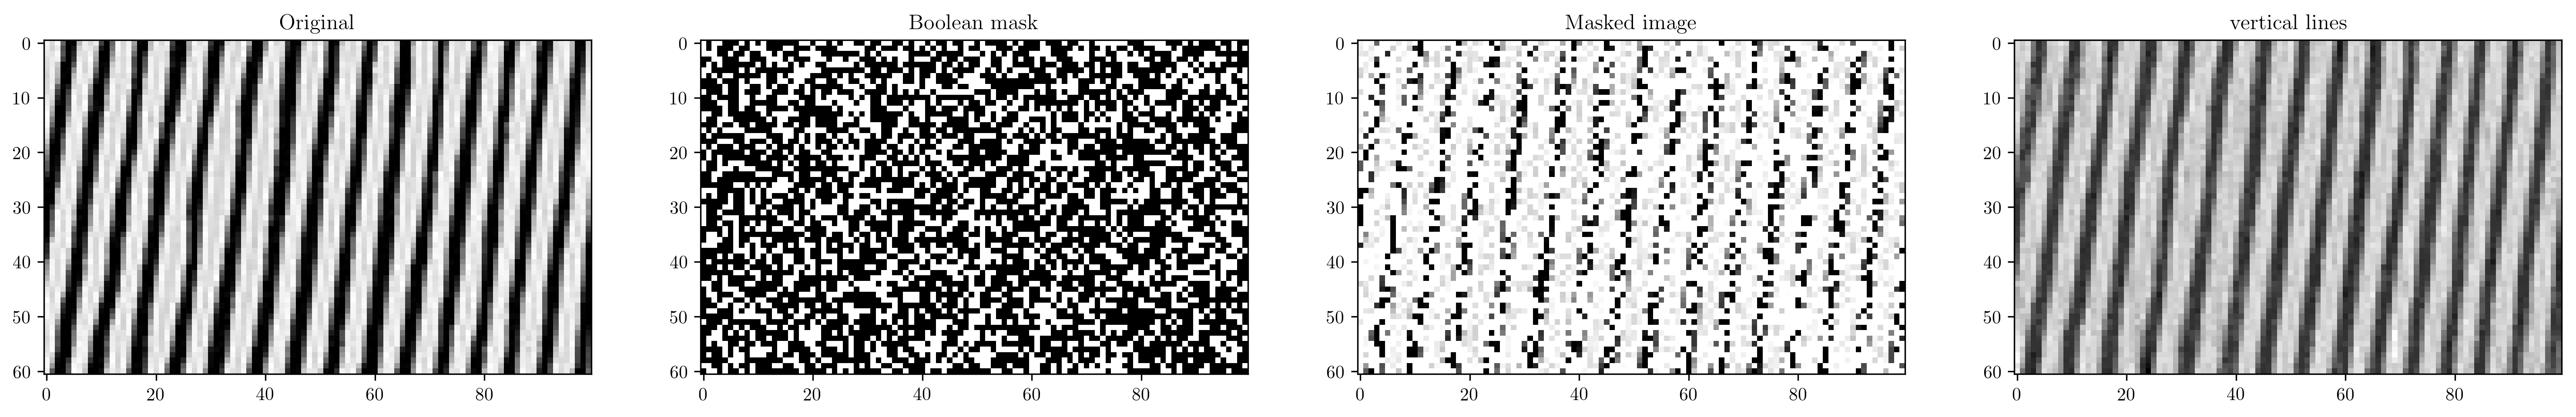
\includegraphics[width=\textwidth]{relativity-vert40.png}
		\caption{Dominant vertical}
		\label{fig:relativity-vert40}
	\end{subfigure}
	\begin{subfigure}{\textwidth}
		\centering
		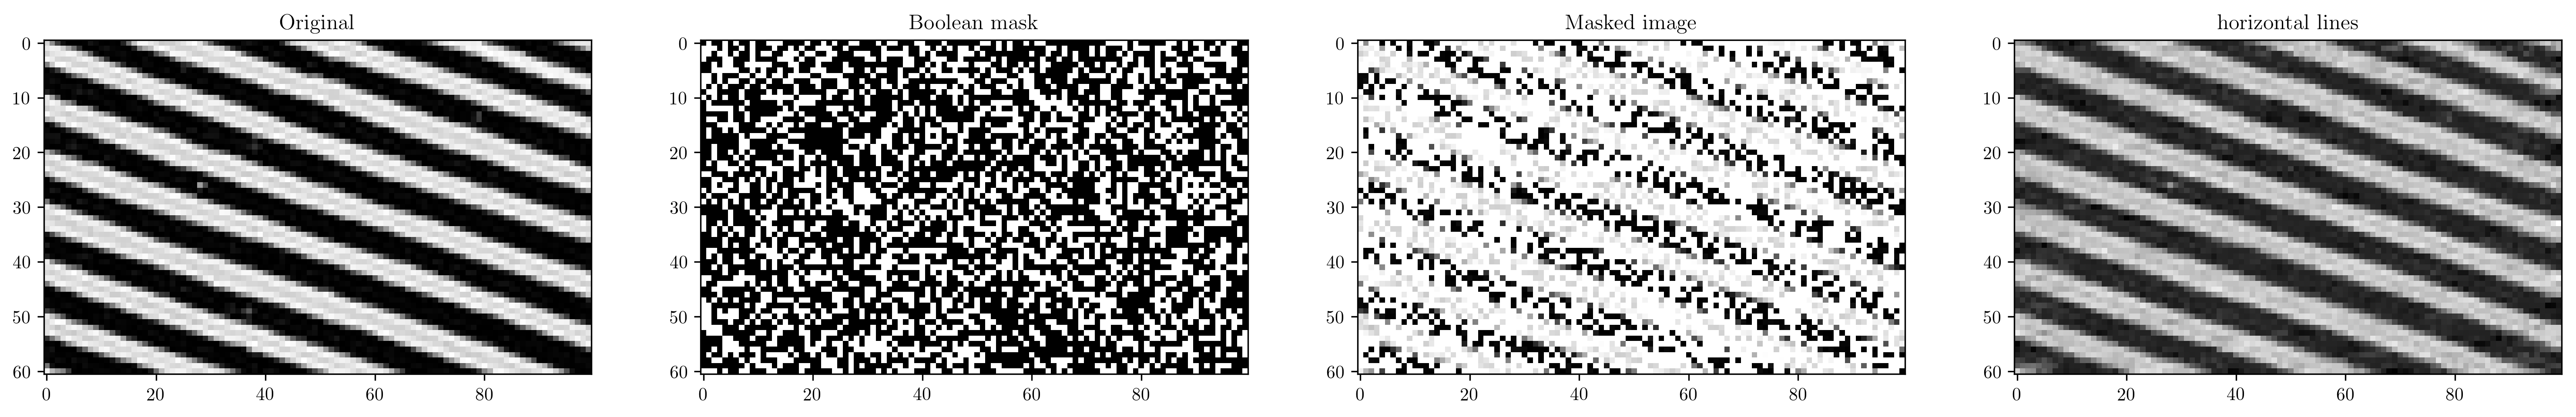
\includegraphics[width=\textwidth]{relativity-horiz40.png}
		\caption{Dominant horizontal}
		\label{fig:relativity-horiz40}
	\end{subfigure}
	\begin{subfigure}{\textwidth}
		\centering
		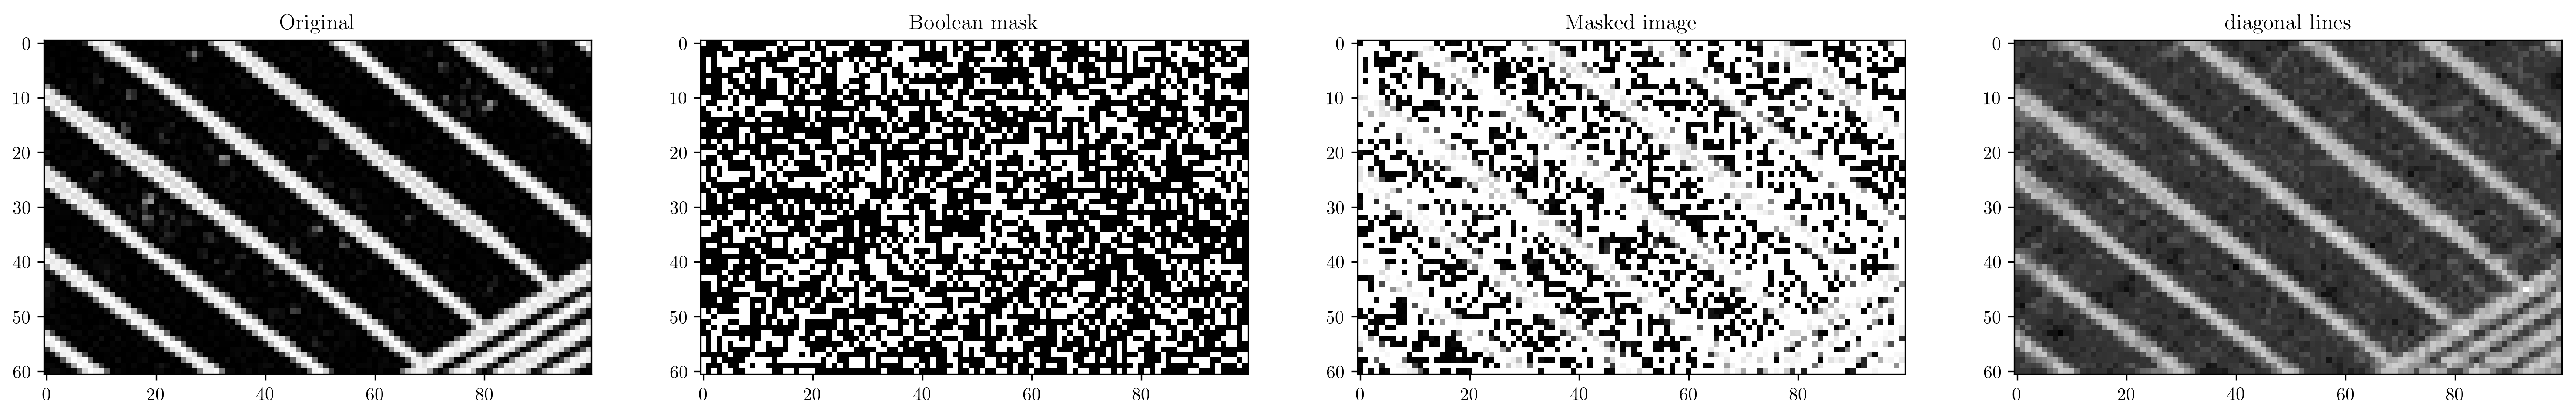
\includegraphics[width=\textwidth]{relativity-diag40.png}
		\caption{Dominant diagonal}
		\label{fig:relativity-diag40}
	\end{subfigure}
	\begin{subfigure}{\textwidth}
		\centering
		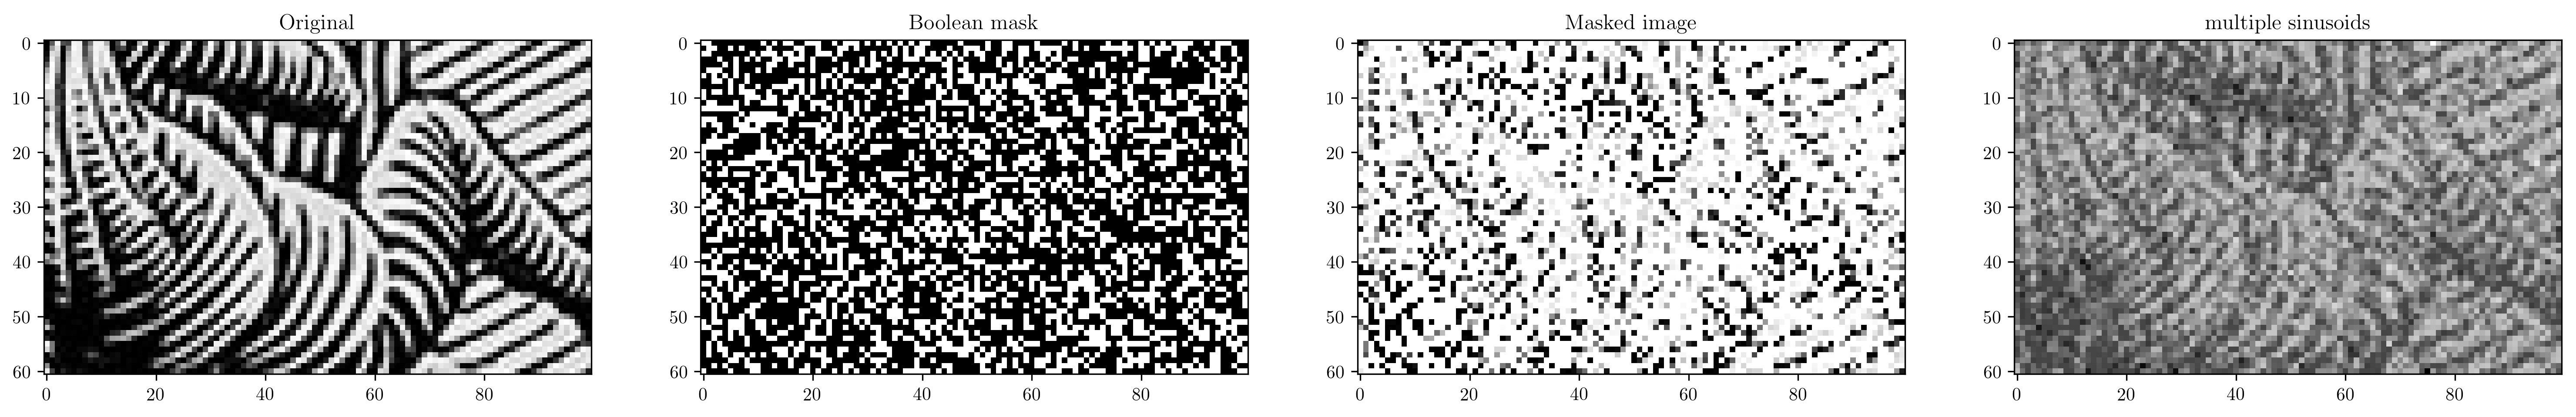
\includegraphics[width=\textwidth]{relativity-mult40.png}
		\caption{Multiple dominant sinusoids}
		\label{fig:relativity-mult40}
	\end{subfigure}
	\begin{subfigure}{\textwidth}
		\centering
		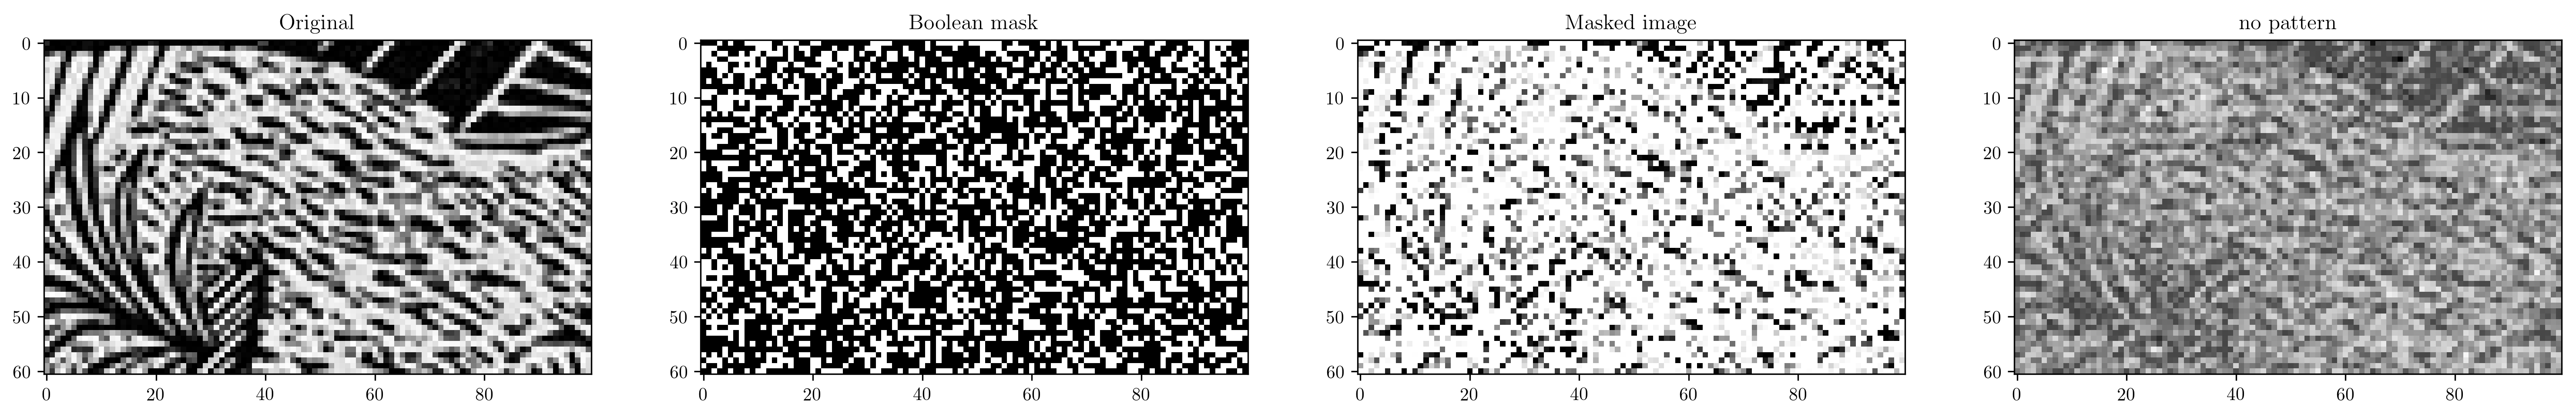
\includegraphics[width=\textwidth]{relativity-high40.png}
		\caption{No dominant pattern}
		\label{fig:relativity-high40}
	\end{subfigure}
	\caption{Extracted and reconstructed patches from \textit{Relativity} using 40\% of samples.}
	\label{fig:relativity-dominant-slices}
\end{figure}


\section{Simultaneous compression \& encryption}
Because of the way compressively sensed images are coded with the sensing matrix, the use of CS as an encryption algorithm arises naturally. Consider the logistic map

\begin{equation}\label{eq:logistic-map}
	x_{n+1} = r x_n \qty(1 - x_n)
\end{equation}

\noindent which is often used as an archetypal example of deterministic chaotic behavior for values of $r \in [3.57, 4]$. In this regime, the sequences produced by varying the initial parameter $x_0$ rapidly diverge from each other. Thus, this can become an encryption system by treating the parameters $r$ and $x_0$ as an encryption key pair, and \eqref{eq:logistic-map} as the hash function.

In application for images, four keys are required: one key pair for each dimension. The construction of the sensing matrix $\bm\Phi$ also differs from the general workflow, and is as follows:

\begin{enumerate}
	\item From \eqref{eq:logistic-map}, generate a sequence of length $2m$ with the initial key pair $r_1$ and $x_{01}$. Discard the first $n$ elements to avoid the transient response and store the latter $n$ elements as a sequence $\vec{s}$.
	\item Explicitly generate the index sequence of $\vec{s}$ and store it as the index sequence $\vec{p} = \qty[0, 1, ..., m-1]$.
	\item Sort $\vec{p}$ according to ascending values of $\vec{s}$.
	\item Generate the first sensing matrix $\bm\Phi_1$ by extracting and stacking rows of a Hadamard matrix of order $N$ indexed by the first $m$ elements of $\vec{p}$, i.e.,
	\begin{equation}\label{eq:construct-hadamard}
		\bm\Phi_1 = \mqty[
			\vec{H}_{p_1} & \vec{H}_{p_2} & \cdots & \vec{H}_{p_M}
		]^\top
	\end{equation}
	\noindent where $\vec{H}_{p_i}$ denotes the $p_i$th row vector of $\vec{H}$.
	\item The second sensing matrix can be constructed using a different key pair $r_2$ and $x_{02}$.
\end{enumerate}

The above steps imply that the image must first be reshaped to have dimensions that are powers of 2. The original image is first reshaped to $256 \times 256$ pixels, and is sparsified by transforming it to the discrete cosine transform (DCT) domain. The desired compressed dimension is set to $m = 192$, corresponding to a compression ratio $m/n = 75\%$, and the keys are set to values of $r_1 = r_2 = 3.99$, $x_{01} = 0.11$, and $x_{02} = 0.24$. Figure \ref{fig:encryption} shows the application of this to the Lena test image (left), its encrypted representation (middle), and the decrypted/reconstructed image (right).

\begin{figure}[htb]
	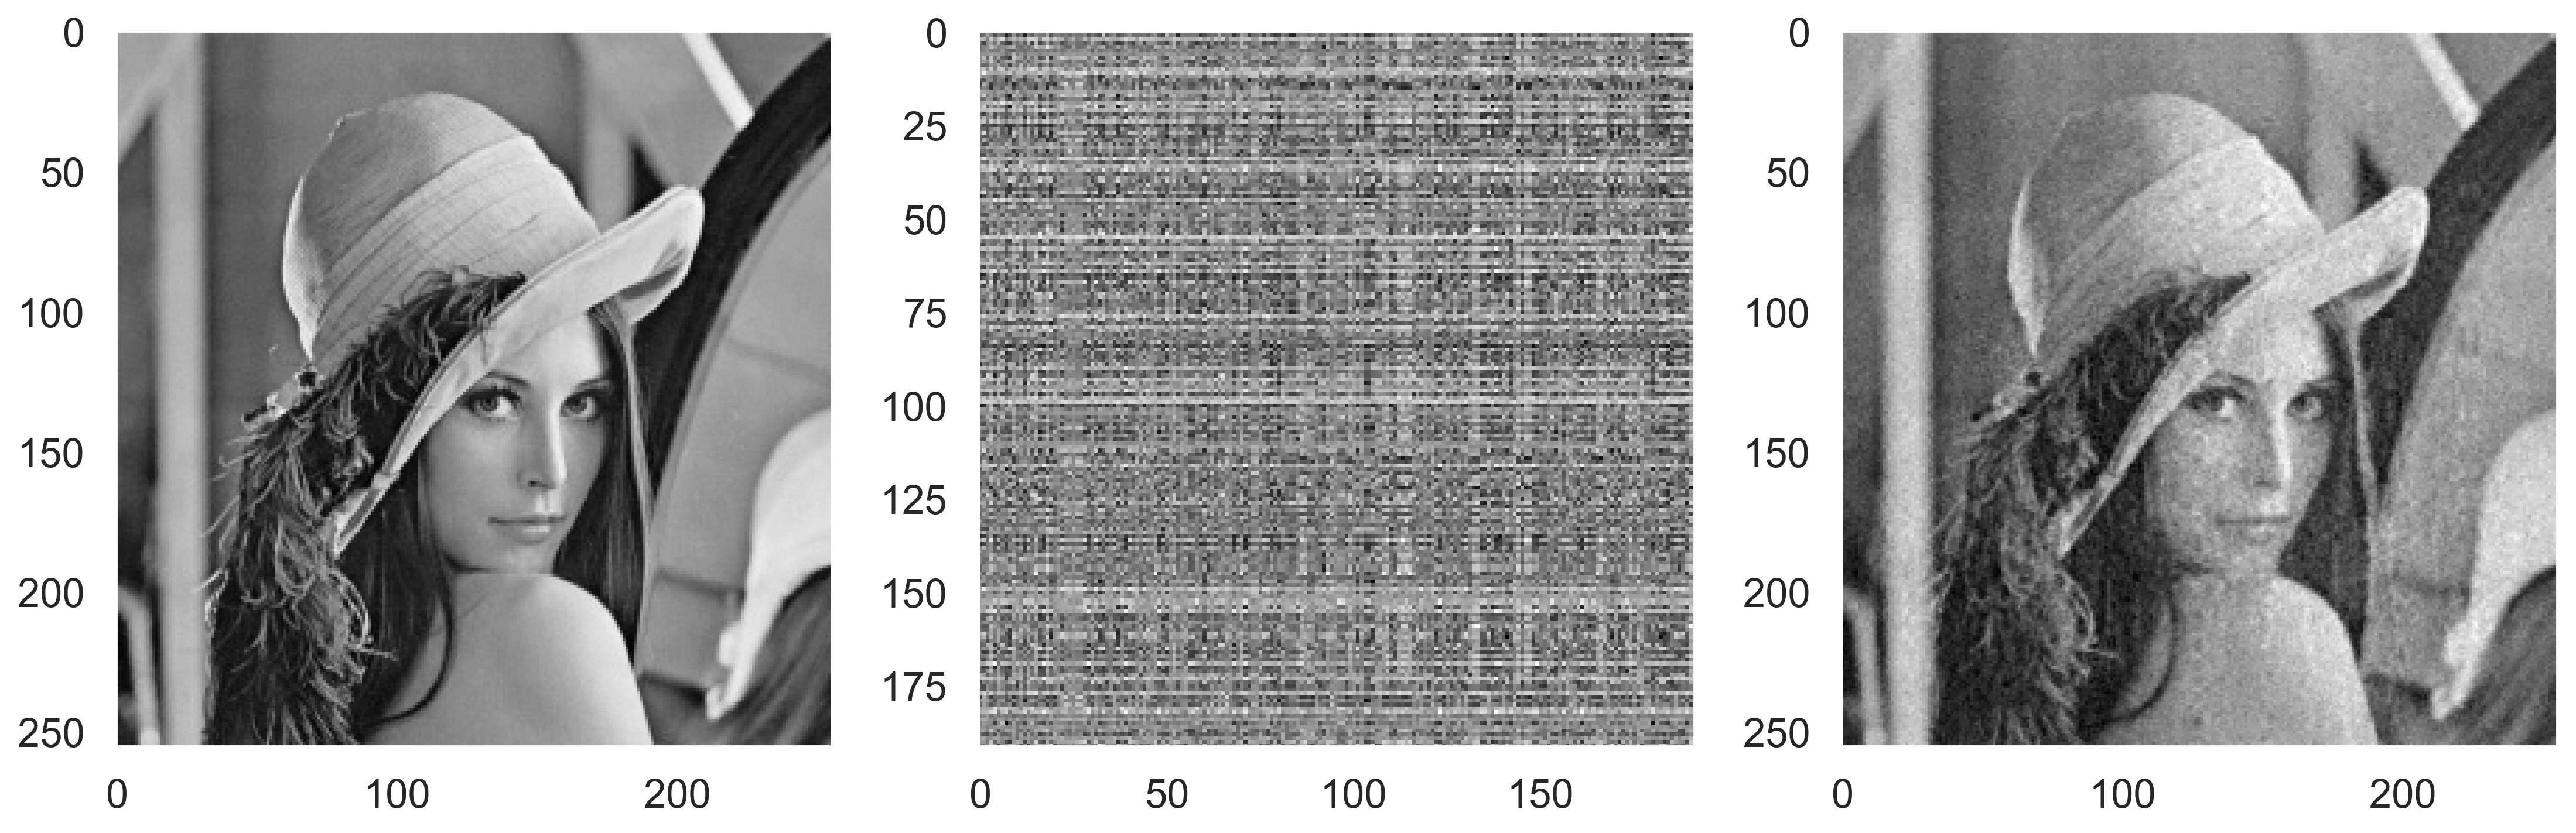
\includegraphics[width=\textwidth]{encryption.png}
	\caption{Simultaneous compression and encryption achieved with compressive sensing: original image (left), encrypted image (middle), and decrypted/reconstructed image (right).}
	\label{fig:encryption}
\end{figure}
\chapter{One-dimensional compressive sensing (1DCS)}
\label{chap:1dcs}
\chapter{Audio compressive sensing}
\label{chap:audio-cs}
In this chapter, I apply CS to audio signals. These type of signals act as the bridge to $N$-dimensional CS as they are one-dimensional when represented in the time domain, but are projected to higher dimensions when represented in another domain, such as the spectrogram/modulation domain. Unlike images, audio signals are more challenging to compressively sample. Due to their relatively higher information density, the effects of undersampling are easily observed.

\section{Test case: Sinusoid redux}
\label{sec:audio-sine}
In this test case, I recorded a guitar playing a single E$_4$ (330 Hz) note at the standard 44.1 kHz sampling rate for 4 seconds. Since the Nyquist rate of the actual signal is 660 Hz, the recording can be downsampled to a practical 8 kHz for processing. The signal waveform and frequency content is shown in Fig.~\ref{fig:guitar-original}. The base frequency is dominant in the frequency spectrum, and several harmonics can be observed. The goal here is to be able to recover the harmonics that have a frequency higher than the compressive sampling rate.

The compressed signal is shown in Fig.~\ref{fig:guitar-compressed}, which was compressively sampled with a quasi-frequency of 1000~Hz (1000 i.i.d.~random samples per second), corresponding to a 12.5\% compression ratio. The waveform envelope still resembles that of the original, but due to the random nature of sampling, the periodicity is not preserved, and is reflected in the seemingly random frequency content.

Following a similar process shown in Chapter \ref{chap:random-cs}, I chose DCT to be the sparse representation domain, and LASSO as the optimization algorithm. The reconstructed signal is shown in Fig.~\ref{fig:guitar-recovered}.For this case, I am concerned only with the frequency components that are recovered, and not so much with the magnitude. Thus, the reconstruction quality can be quantified using the cosine similarity

\begin{equation}
	\label{eq:cossim}
	\mathrm{similarity} = \cos\theta = \frac{\vec{x} \cdot \bm\hat{\vec{x}}}{\norm{\vec{x}}_2 \norm{\bm\hat{\vec{x}}}_2}
\end{equation}

\noindent which allows us to compare two signals' frequency content directly in the time domain. A cosine similarity value of 0.8 and above indicates acceptable quality; a value of 1.0 indicates perfect reconstruction.

\begin{figure}[htb]
	\centering
	\begin{subfigure}{\textwidth}
		\centering
		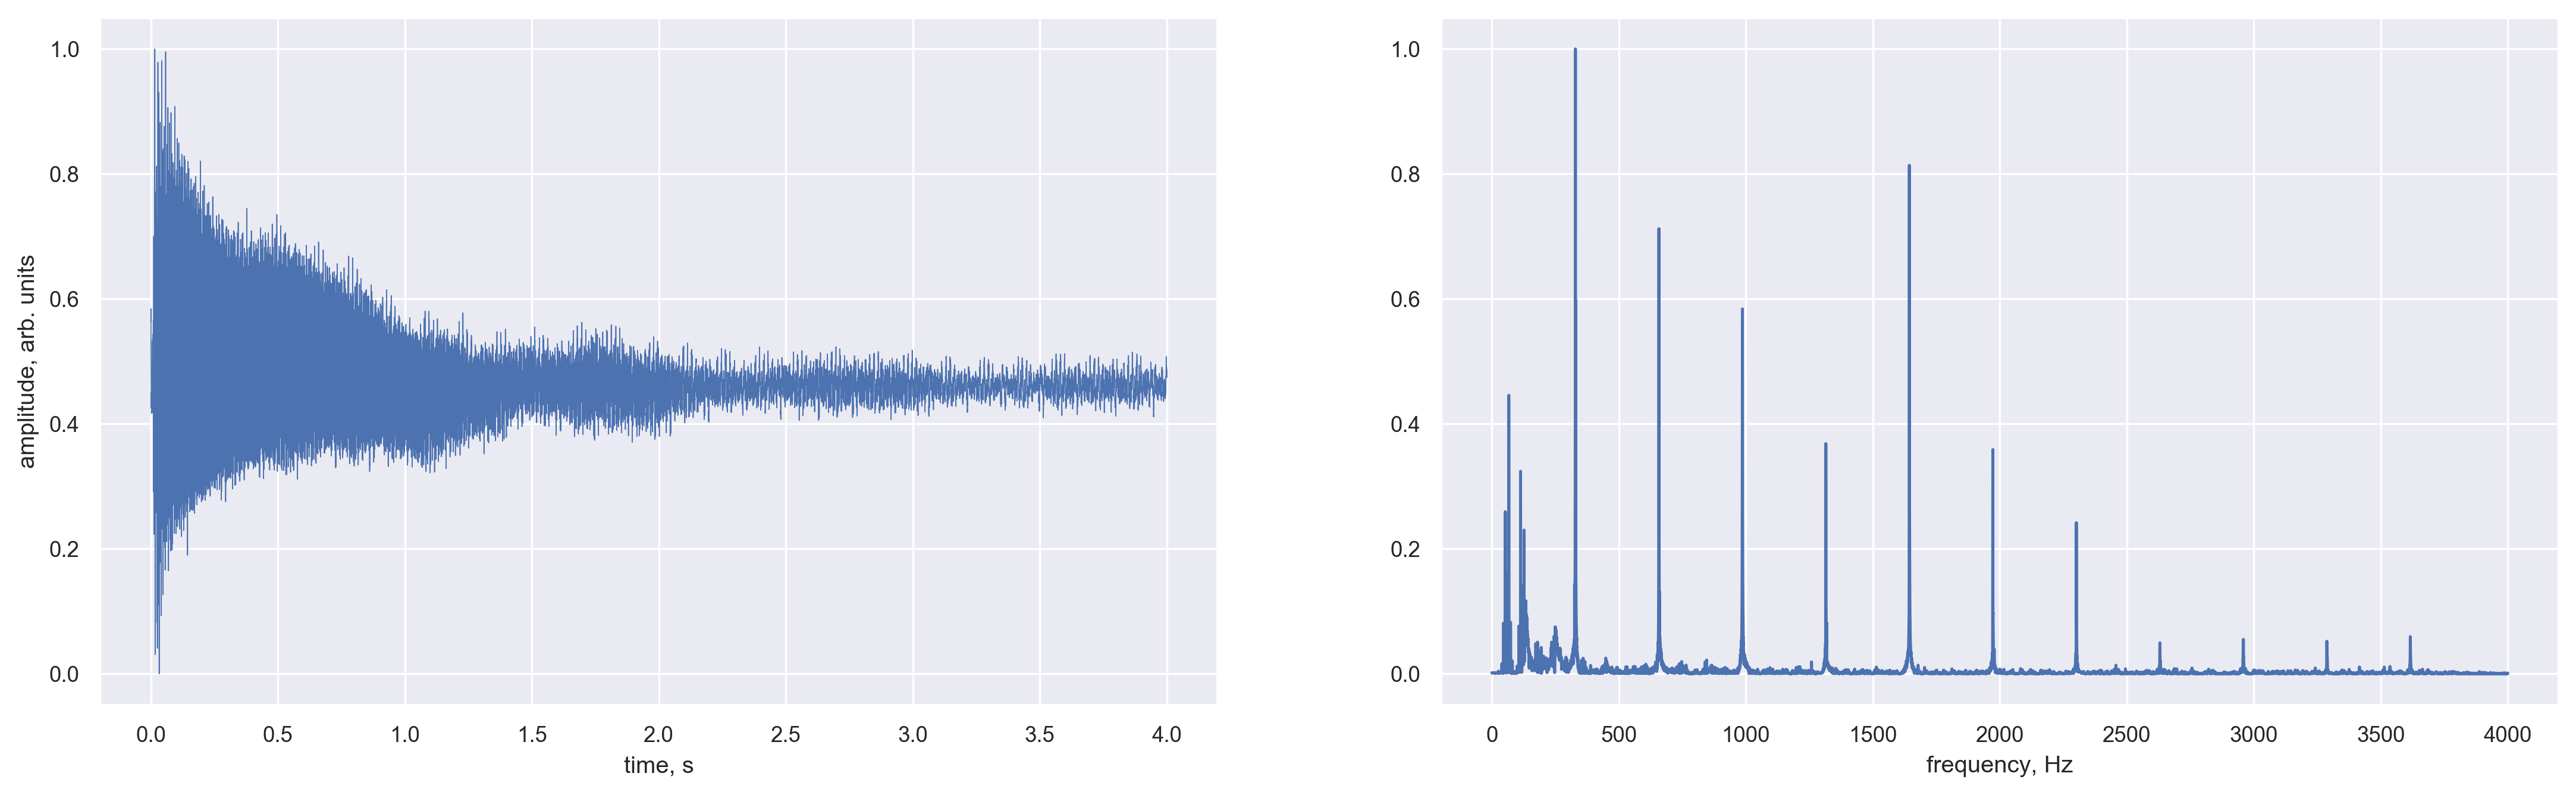
\includegraphics[width=\textwidth]{E1_orig.png}
		\caption{Original}
		\label{fig:guitar-original}
	\end{subfigure}
	\begin{subfigure}{\textwidth}
		\centering
		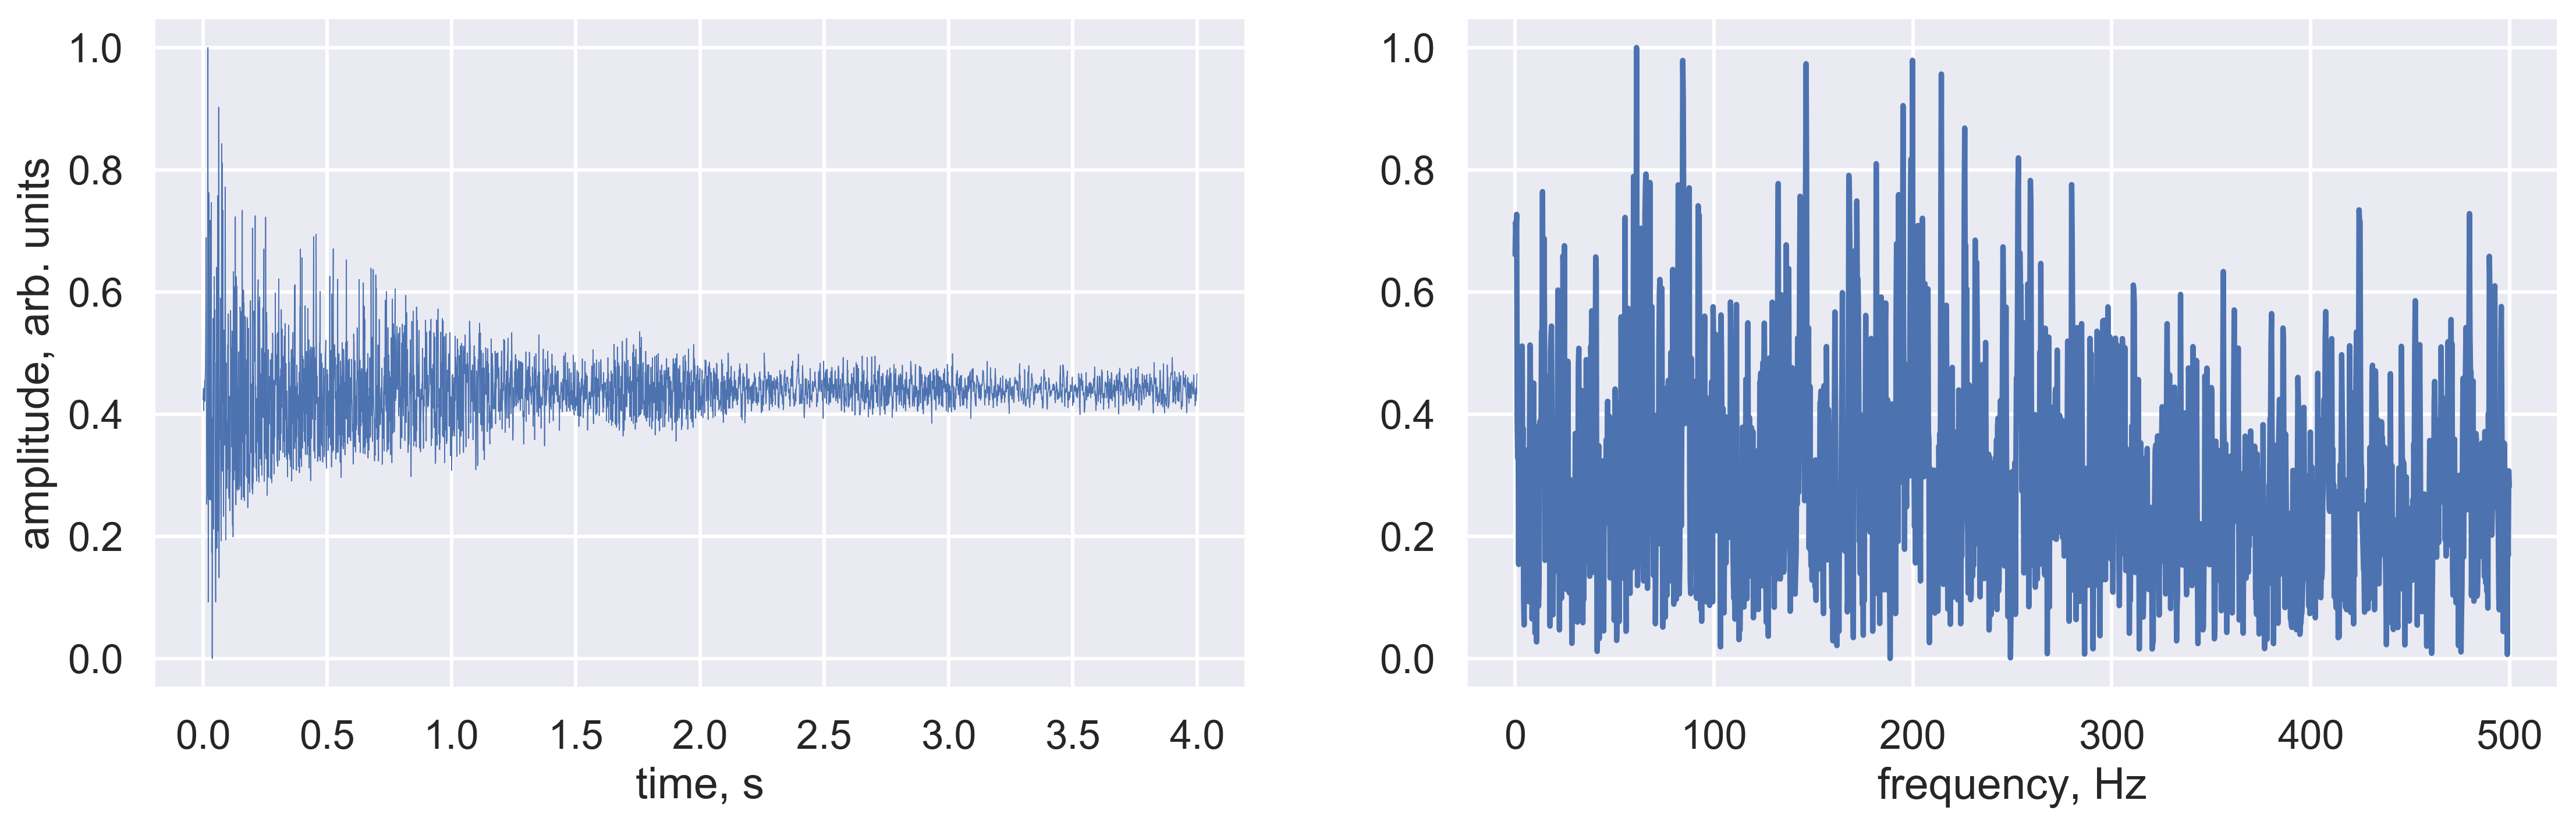
\includegraphics[width=\textwidth]{E1_comp.png}
		\caption{Compressed}
		\label{fig:guitar-compressed}
	\end{subfigure}
	\begin{subfigure}{\textwidth}
		\centering
		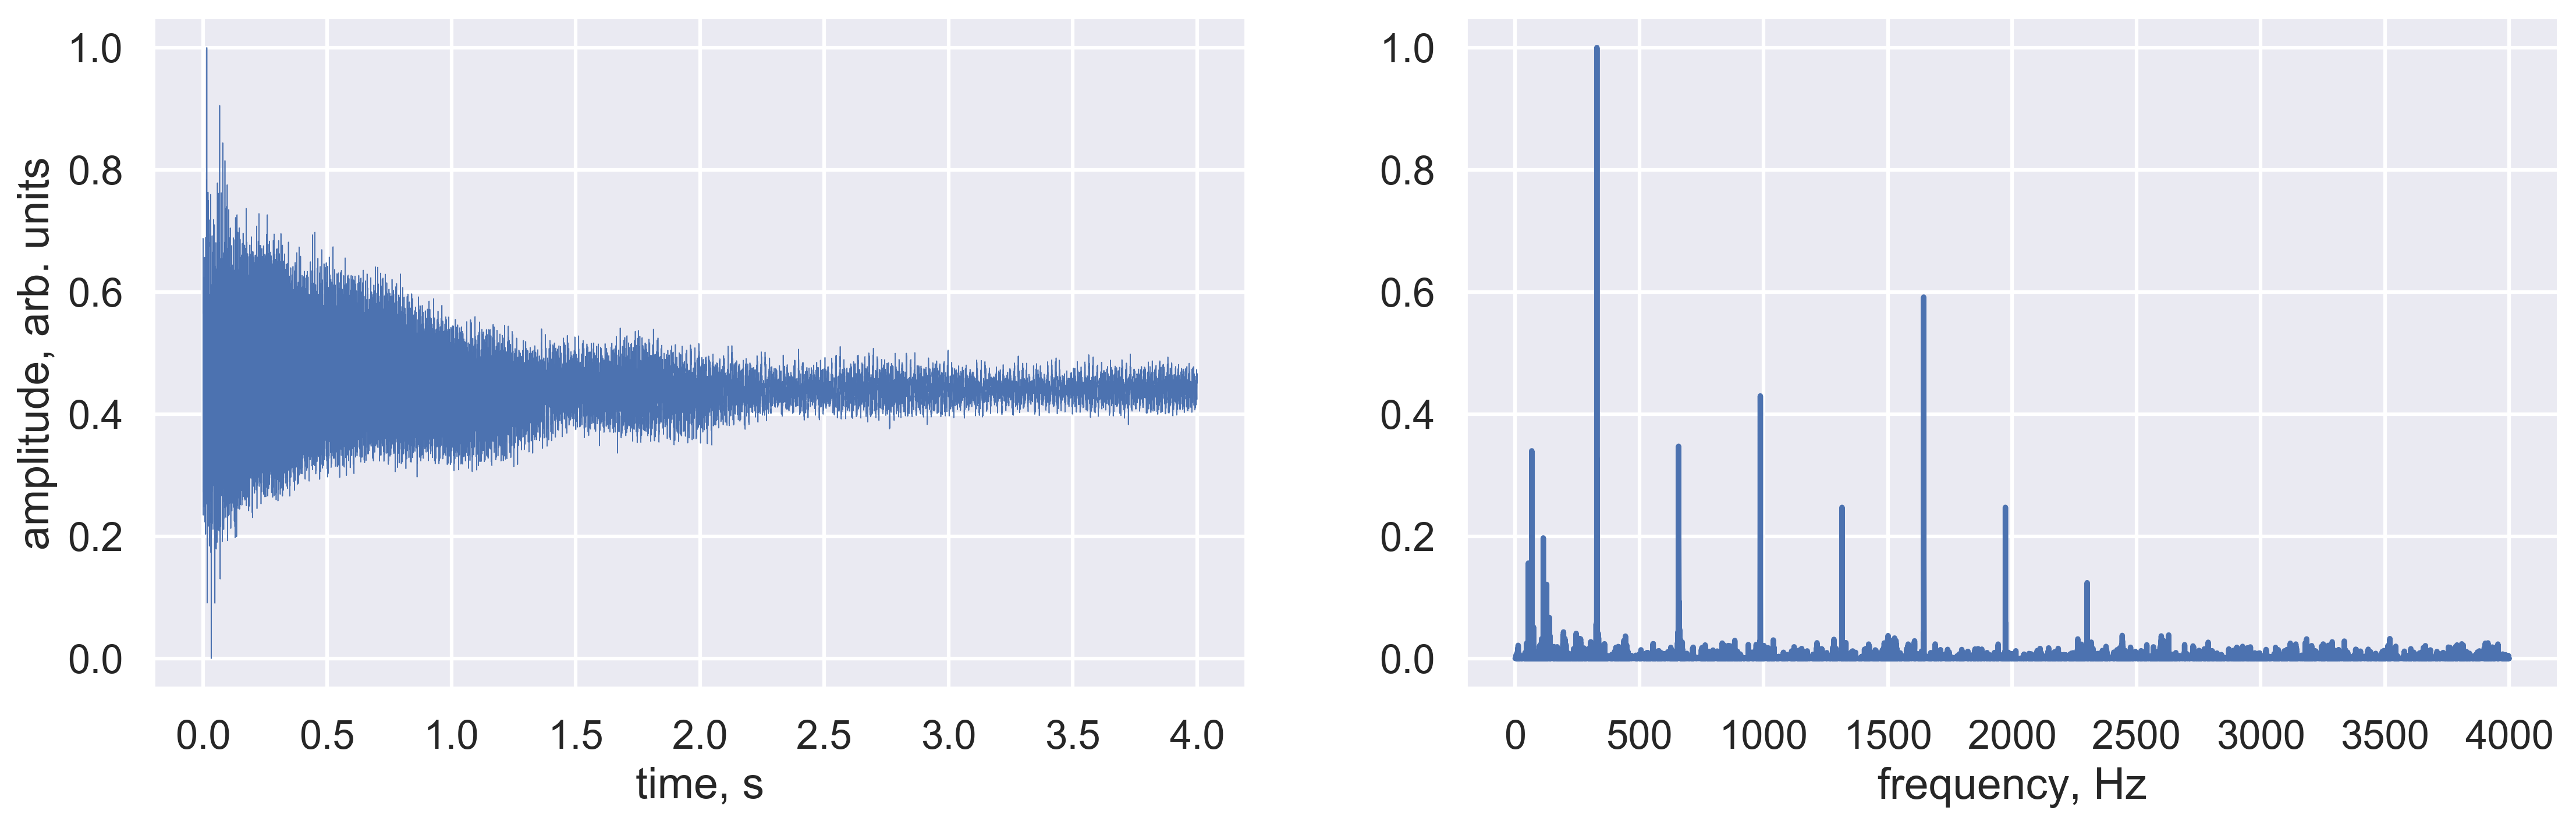
\includegraphics[width=\textwidth]{E1_recov.png}
		\caption{Recovered}
		\label{fig:guitar-recovered}
	\end{subfigure}
	\caption{330 Hz guitar signal representation in the time domain (left column) and frequency domain (right column).}
	\label{fig:guitar}
\end{figure}


\section{Comparison of algorithms}
\label{sec:audio-algorithms}
Following the same procedure as the previous section, my aim now is to compare the performance of three different reconstruction algorithms in terms of average runtime and reconstruction quality. The algorithms used are LASSO and OMP, which were described in Chapter~\ref{chap:theory}. Additionally, the Smoothed L$_0$ Norm (SL0) \cite{Mohimani2009} is used, which approximates the $\ell_0$ norm using a Gaussian of the form

\begin{equation}
	\label{eq:sl0}
	\lim_{\sigma \rightarrow 0} x \exp\qty(-\frac{x^2}{2\sigma^2}).
\end{equation}

While all algorithms have polynomial time complexity \cite{Efron2004,Sturm2012,Xiang2019}, OMP shows the worst scaling with respect to time; LASSO and SL0 show similar performance over time (Fig.~\ref{fig:guitar-runtime}). In terms of reconstruction quality (cosine similarity), LASSO is able to breach the 0.8 threshold at 30\% compression ratio, while SL0 achieves this at 50\% compression. On the other hand, OMP shows a nonlinear trend with a large error, which is indicative of unstable performance for low compression ratios (Fig.~\ref{fig:guitar-cossim}).

\begin{figure}[htb]
	\centering
	\begin{subfigure}{0.49\textwidth}
		\centering
		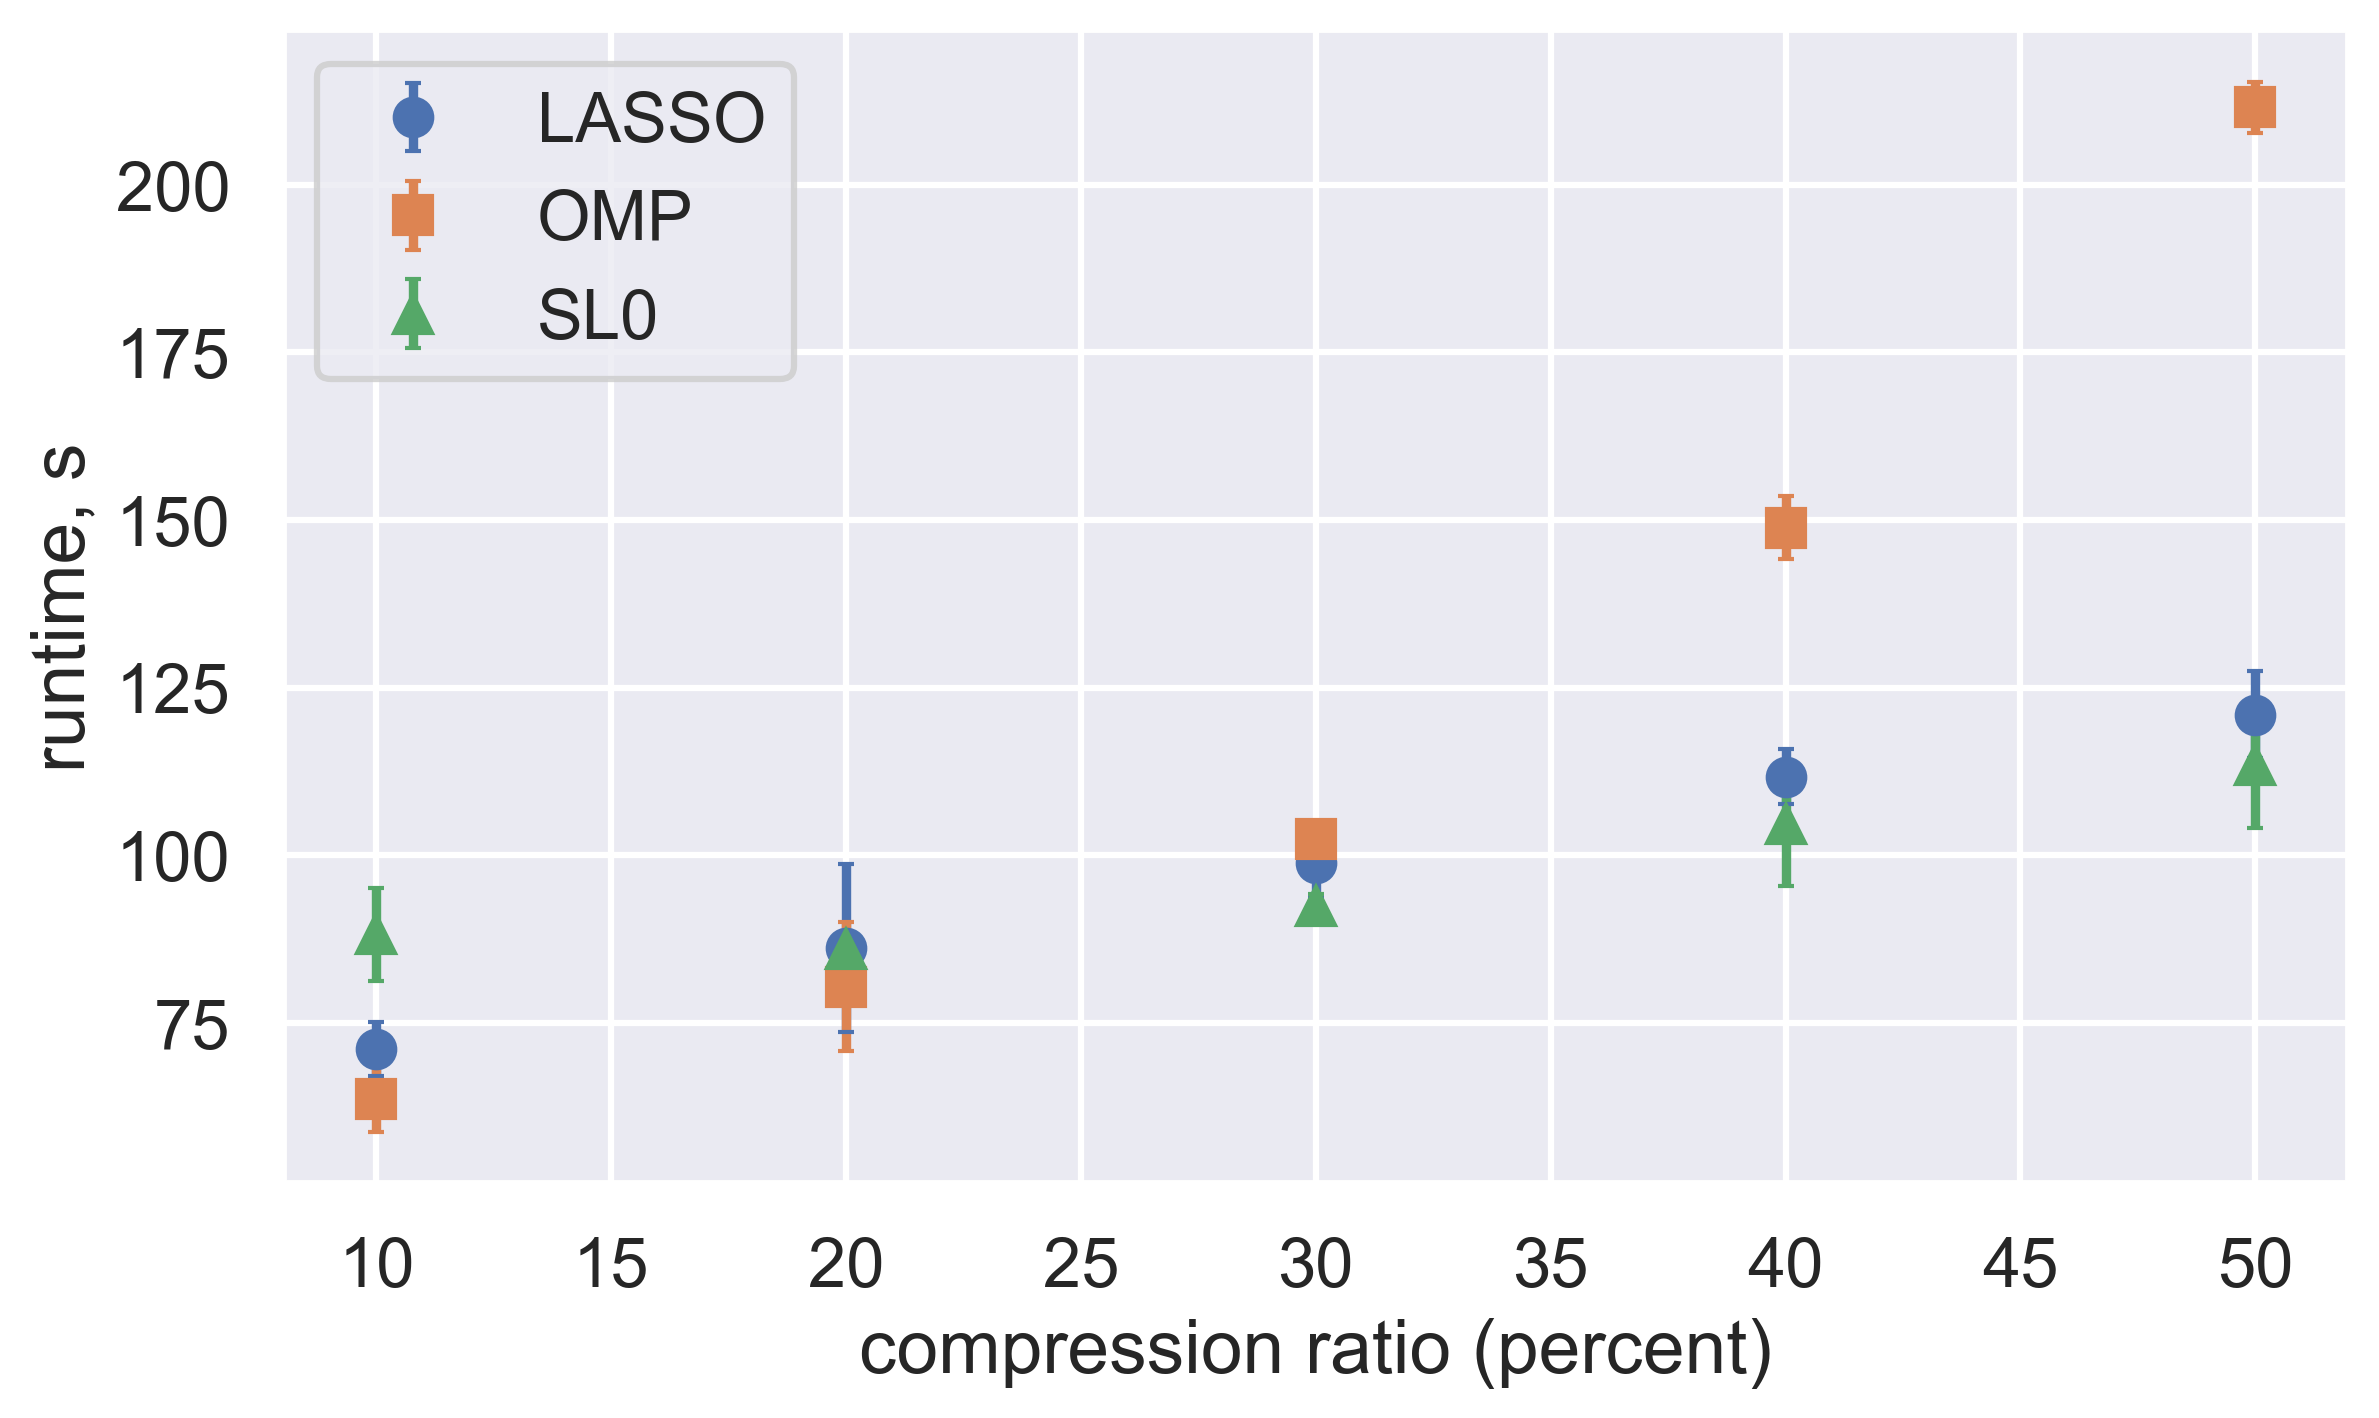
\includegraphics[width=\textwidth]{E1_processtime.png}
		\caption{Runtime}
		\label{fig:guitar-runtime}
	\end{subfigure}
	\begin{subfigure}{0.49\textwidth}
		\centering
		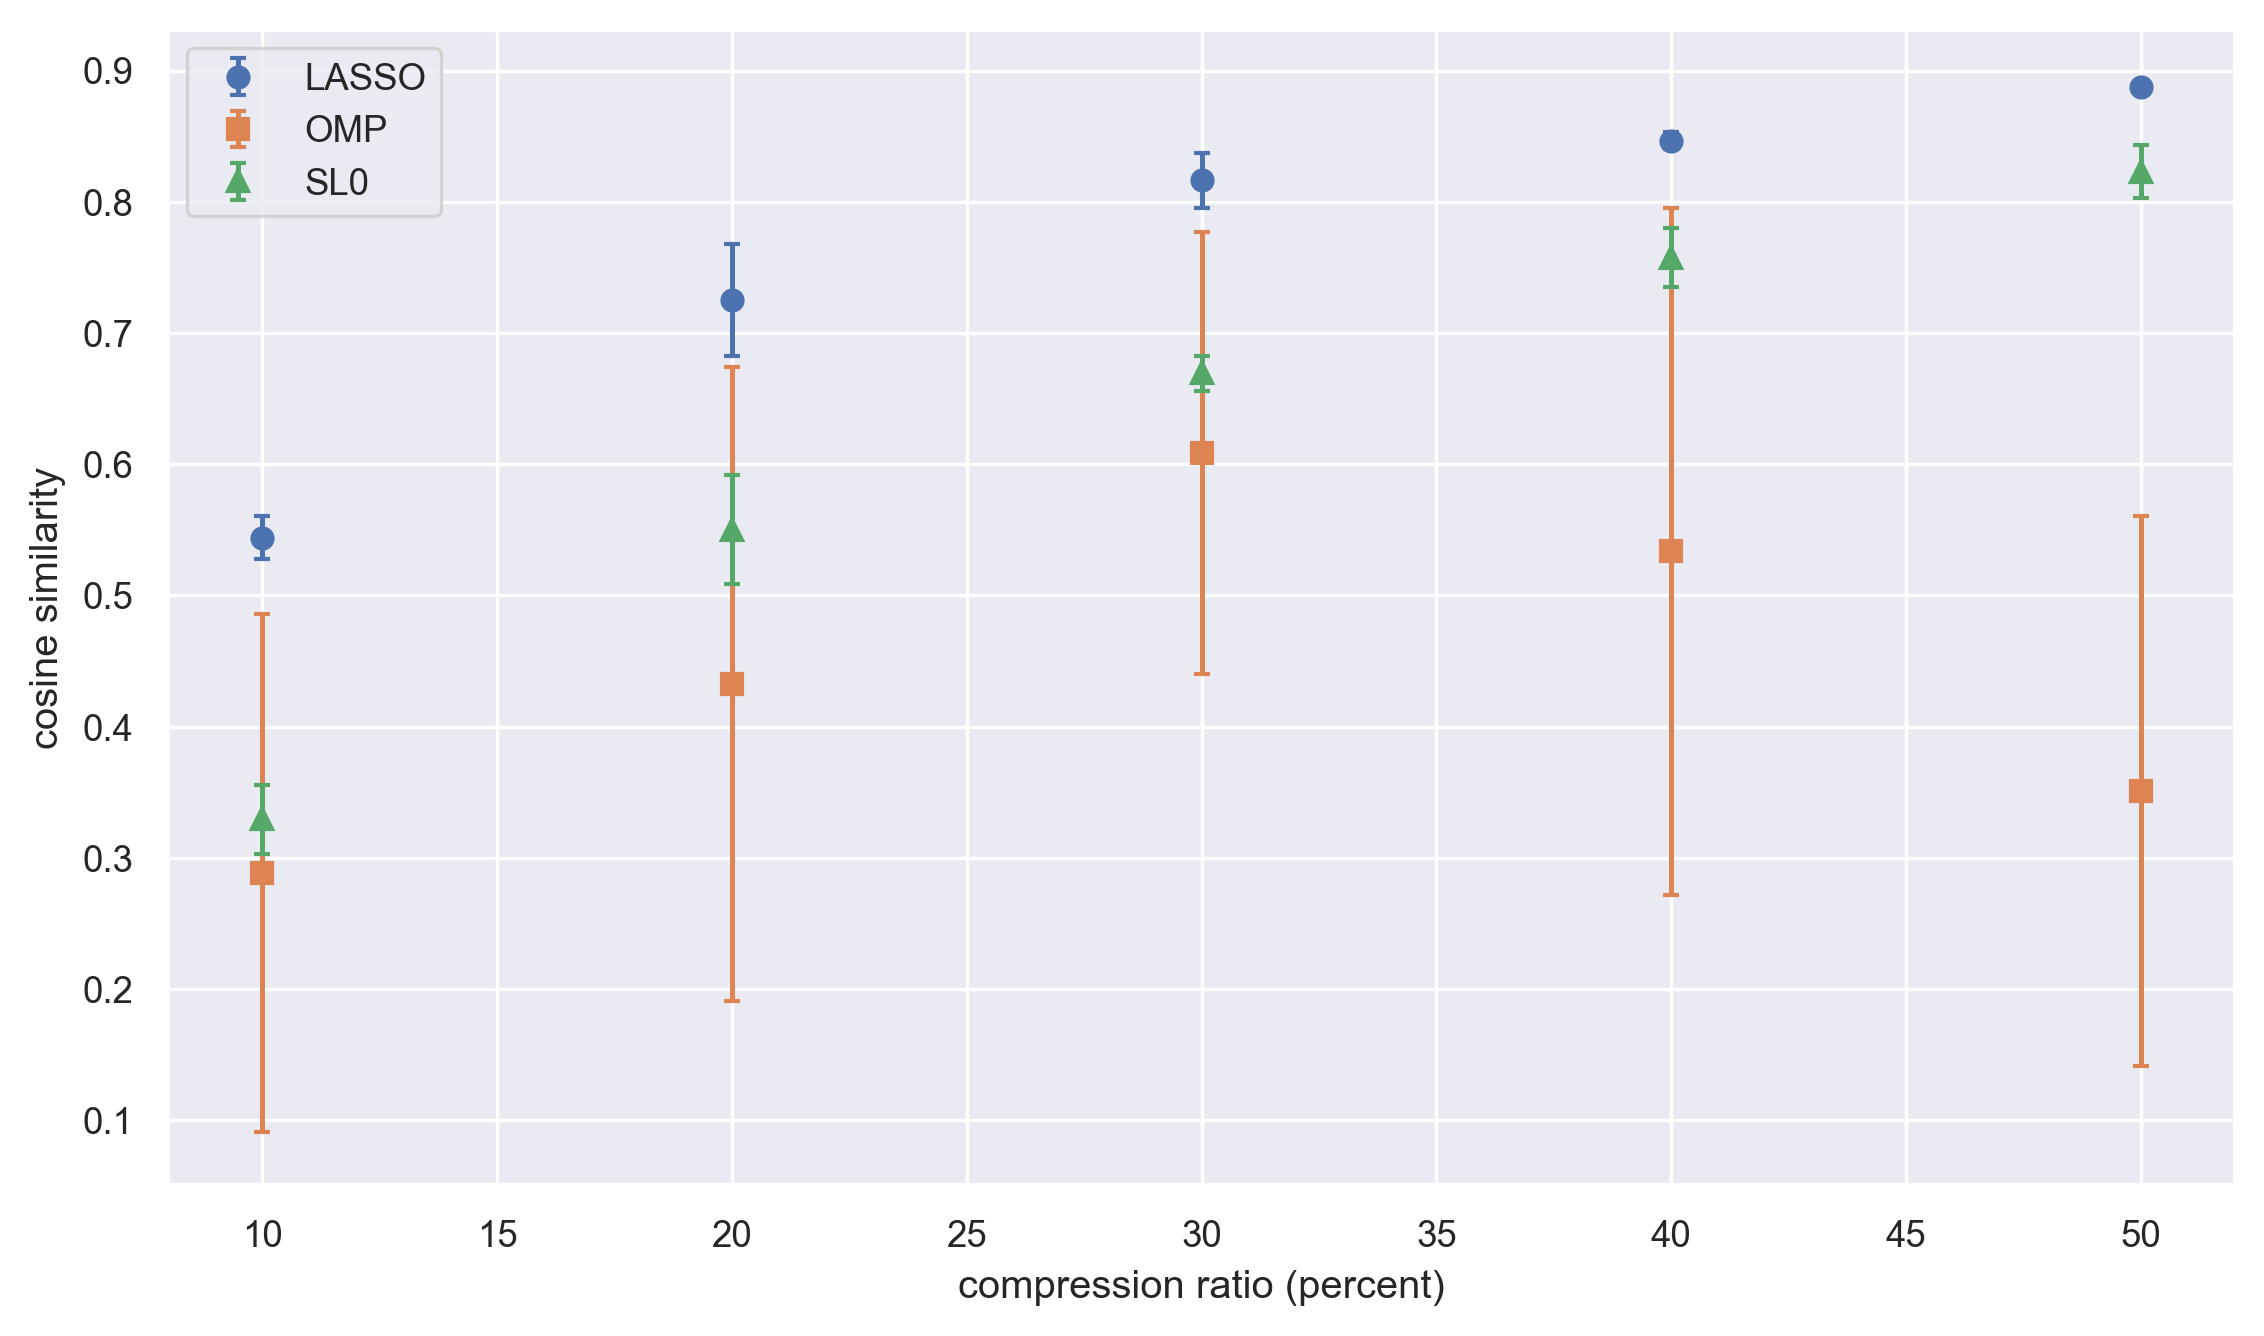
\includegraphics[width=\textwidth]{E1_cossim.png}
		\caption{Reconstruction quality}
		\label{fig:guitar-cossim}
	\end{subfigure}
	\caption{Evaluation of the performance of LASSO, OMP, and SL0 in reconstructing the guitar signal shown in Fig.~\ref{fig:guitar}, in terms of runtime (a) and cosine similarity (b).}
	\label{fig:guitar-algorithms}
\end{figure}


\section{Speech}
\label{sec:audio-speech}
In order to show its practical merits, we will inevitably have to deal with increasingly large and complex signals. Audio recordings containing speech will encompass a wide range of frequencies, so such signals can only be downsampled so much before essential information is lost to aliasing. Unlike images, large audio signals cannot simply be chopped into smaller, manageable pieces. The effects of aliasing are amplified due to the high information density, and CS' violation of periodic constraints introduce artifacts in the vicinity of where the signal was sliced. This is the motivation for transforming the signal first into the modulation domain (spectrogram).

\subsection{Sparse transformation}
\label{ssec:audio-speech-sparse}
In obtaining the spectrogram representation, first define a short length sampling window, typically only a few milliseconds in duration, as well as the overlap between adjacent frames. The latter is crucial in suppressing boundary artifacts as it ensures that some information from the current measurement is carried over to the next measurement. The signal is then divided into frames by sliding this window across the entire signal. Each frame is multiplied with a window function; in this case, I used the Hann window, defined as

\begin{equation}
	\label{eq:hann-window}
	w[n] = \sin^2\qty(\frac{\pi n}{N})
\end{equation}

\noindent where $N + 1$ is the length of the window, and $n: 0 \leq n \leq N$ is the frame index. Finally, each frame undergoes a Fourier transformation. The entire process is also called a short-time Fourier transform, and is summarized as

\begin{equation}
	\label{eq:stft}
	X(\omega, p) = \sum_{p=0}^{P-1} x[p] w[p - kR] e^{-i\omega p}
\end{equation}

\noindent where $x[p]$ is the $p$th signal frame, $w[p - kR]$ is the window function with hop size $R$ and time index $k$, and $\omega$ is the angular frequency.

\subsection{Pre-processing}
\label{ssec:audio-speech-preprocess}
Test signals were obtained from the TIMIT Acoustic-Phonetic Continuous Speech Corpus \cite{timit}, which contains speech recordings in \texttt{WAV} format. The recordings are of English speakers grouped by region, sex, and unique spoken sentence. All files have a sampling rate of 16 kHz and are, on average, 3 seconds long. I chose a test signal at random, specifically the \texttt{DR8/MJLN0/SA1.wav} file. This indicates that the speaker was from dialect region 8 (nomadic), was male with speaker code \texttt{JLN0}, and spoke unique sentence \texttt{SA1}, which reads

\begin{quotation}
	She had your dark suit in greasy wash water all year.
\end{quotation}

Before proceeding, I downsampled the file to 8 kHz. The representation of the signal in the time and modulation domains are shown in Fig.~\ref{fig:speech-original}.

\begin{figure}[htb]
	\centering
	\begin{subfigure}{0.49\textwidth}
		\centering
		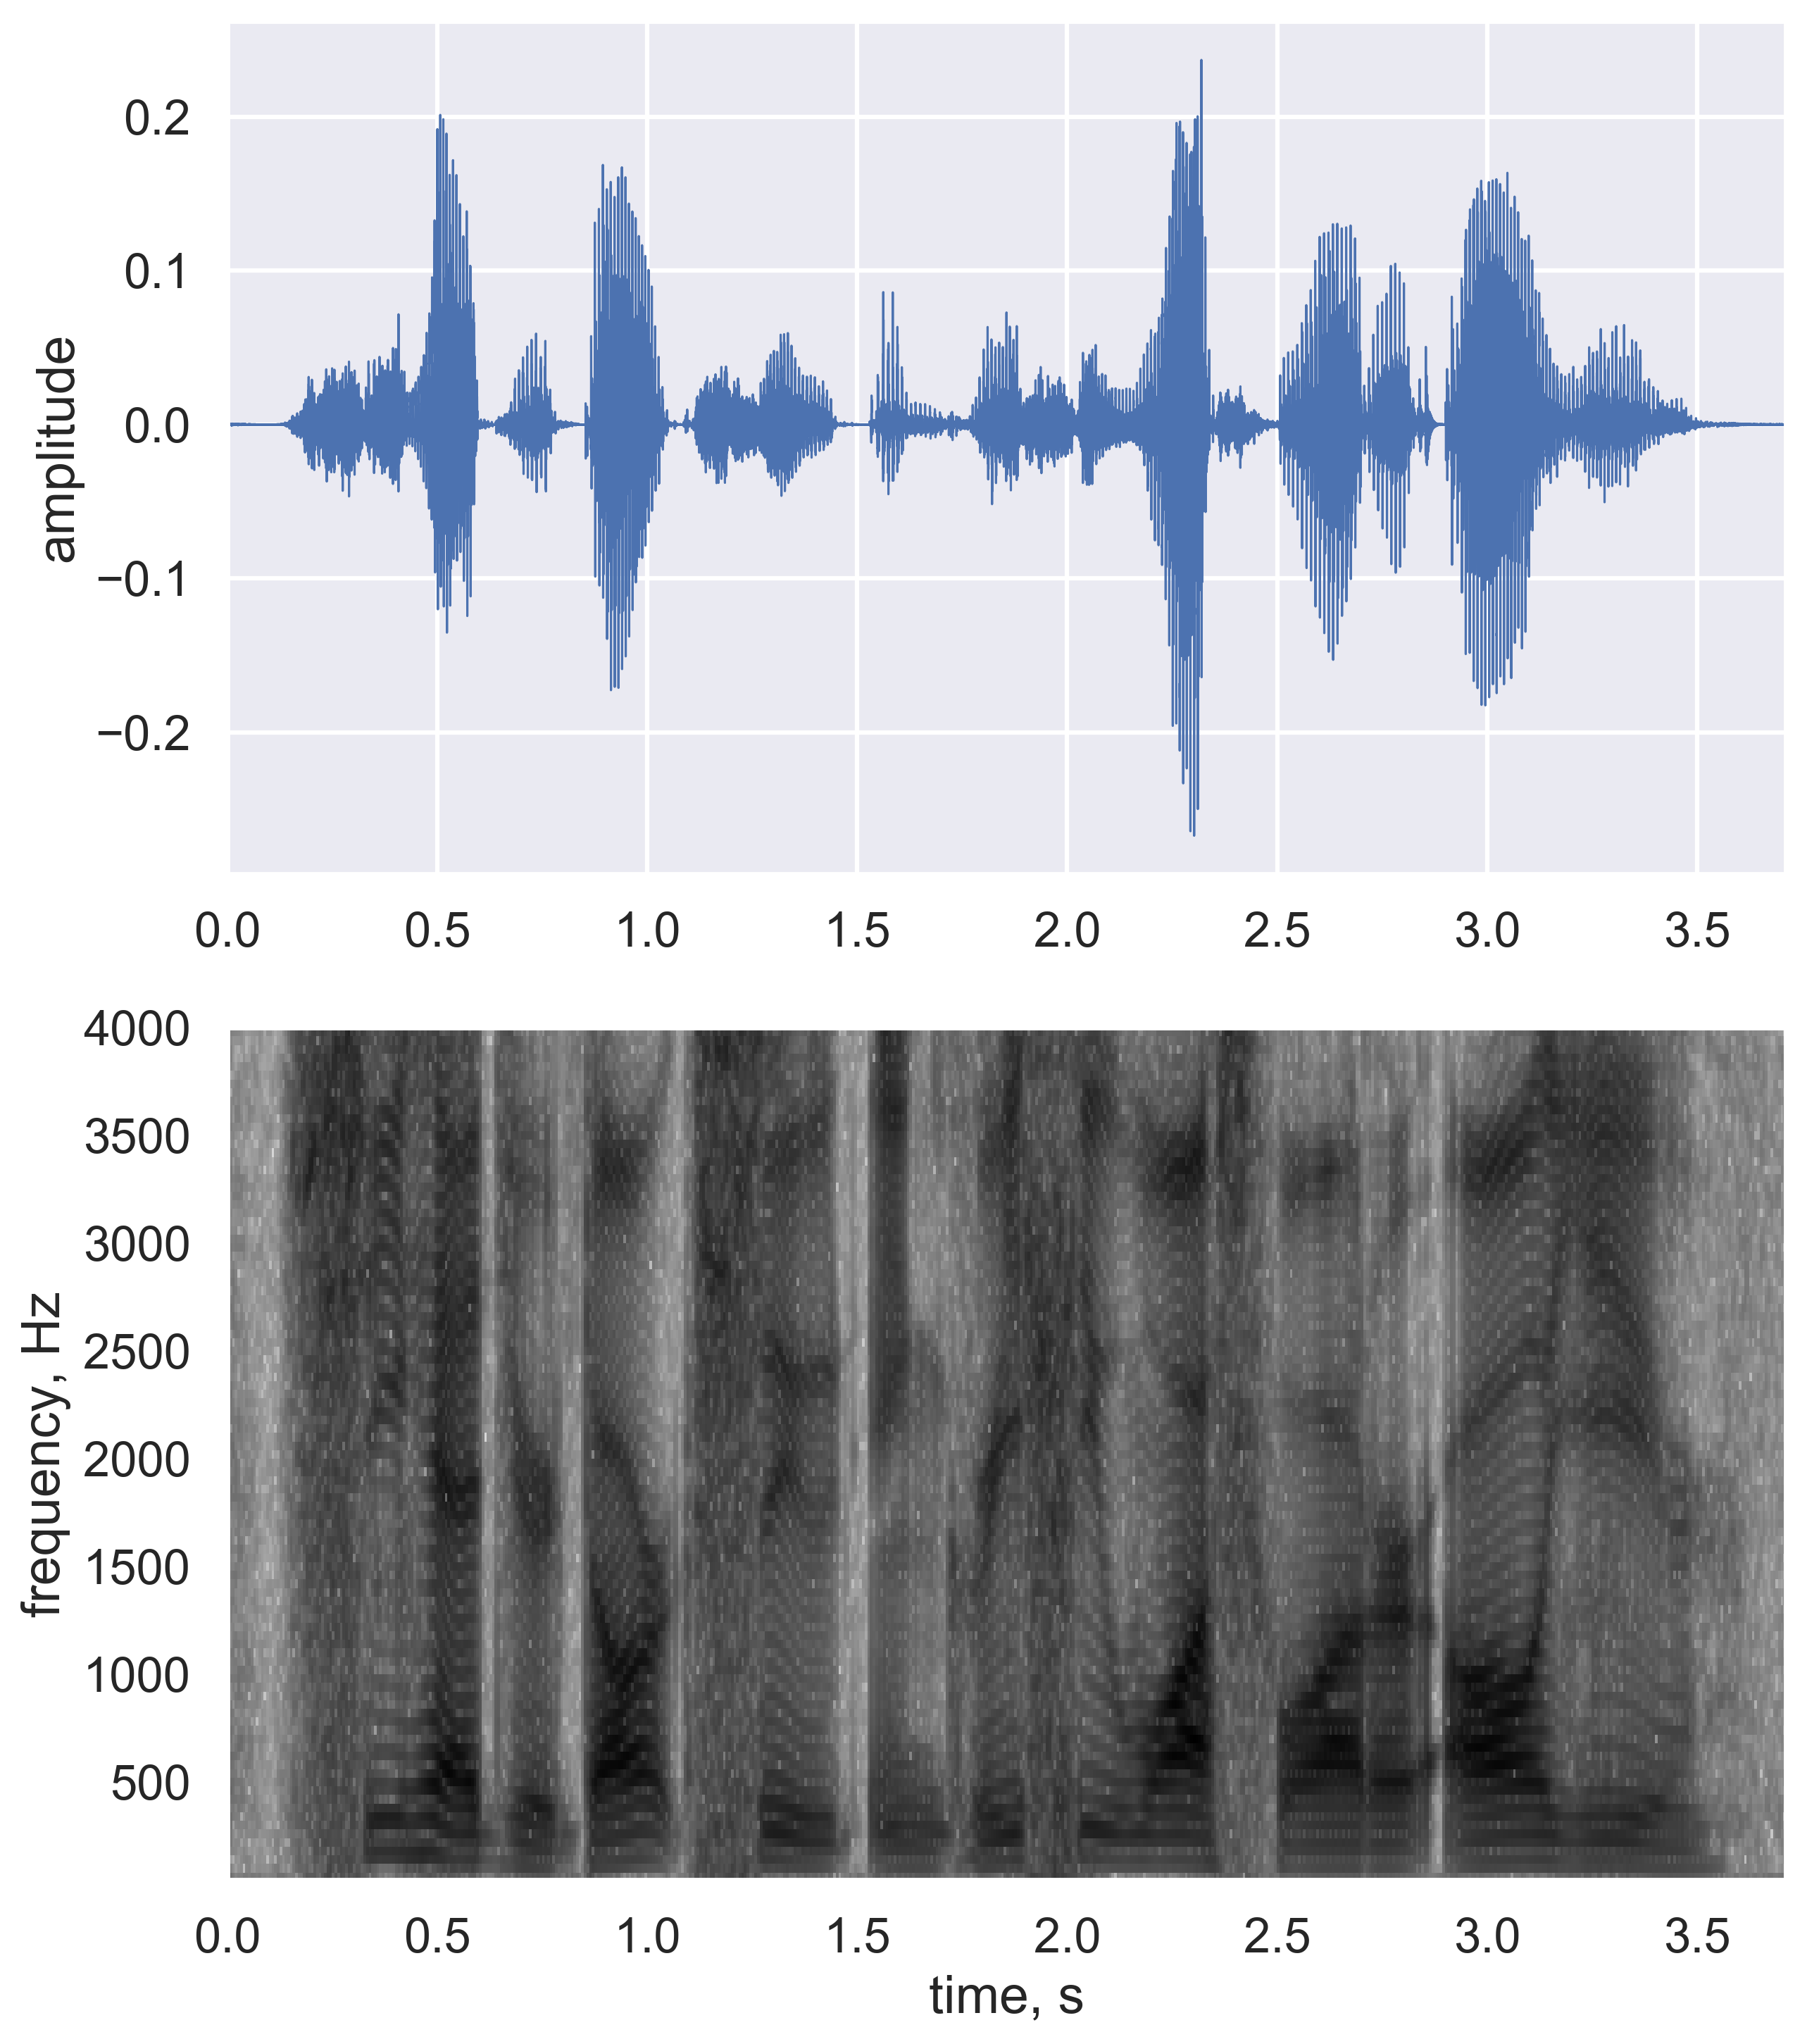
\includegraphics[width=\textwidth]{speech_original.png}
		\caption{Original}
		\label{fig:speech-original}
	\end{subfigure}
	\begin{subfigure}{0.49\textwidth}
		\centering
		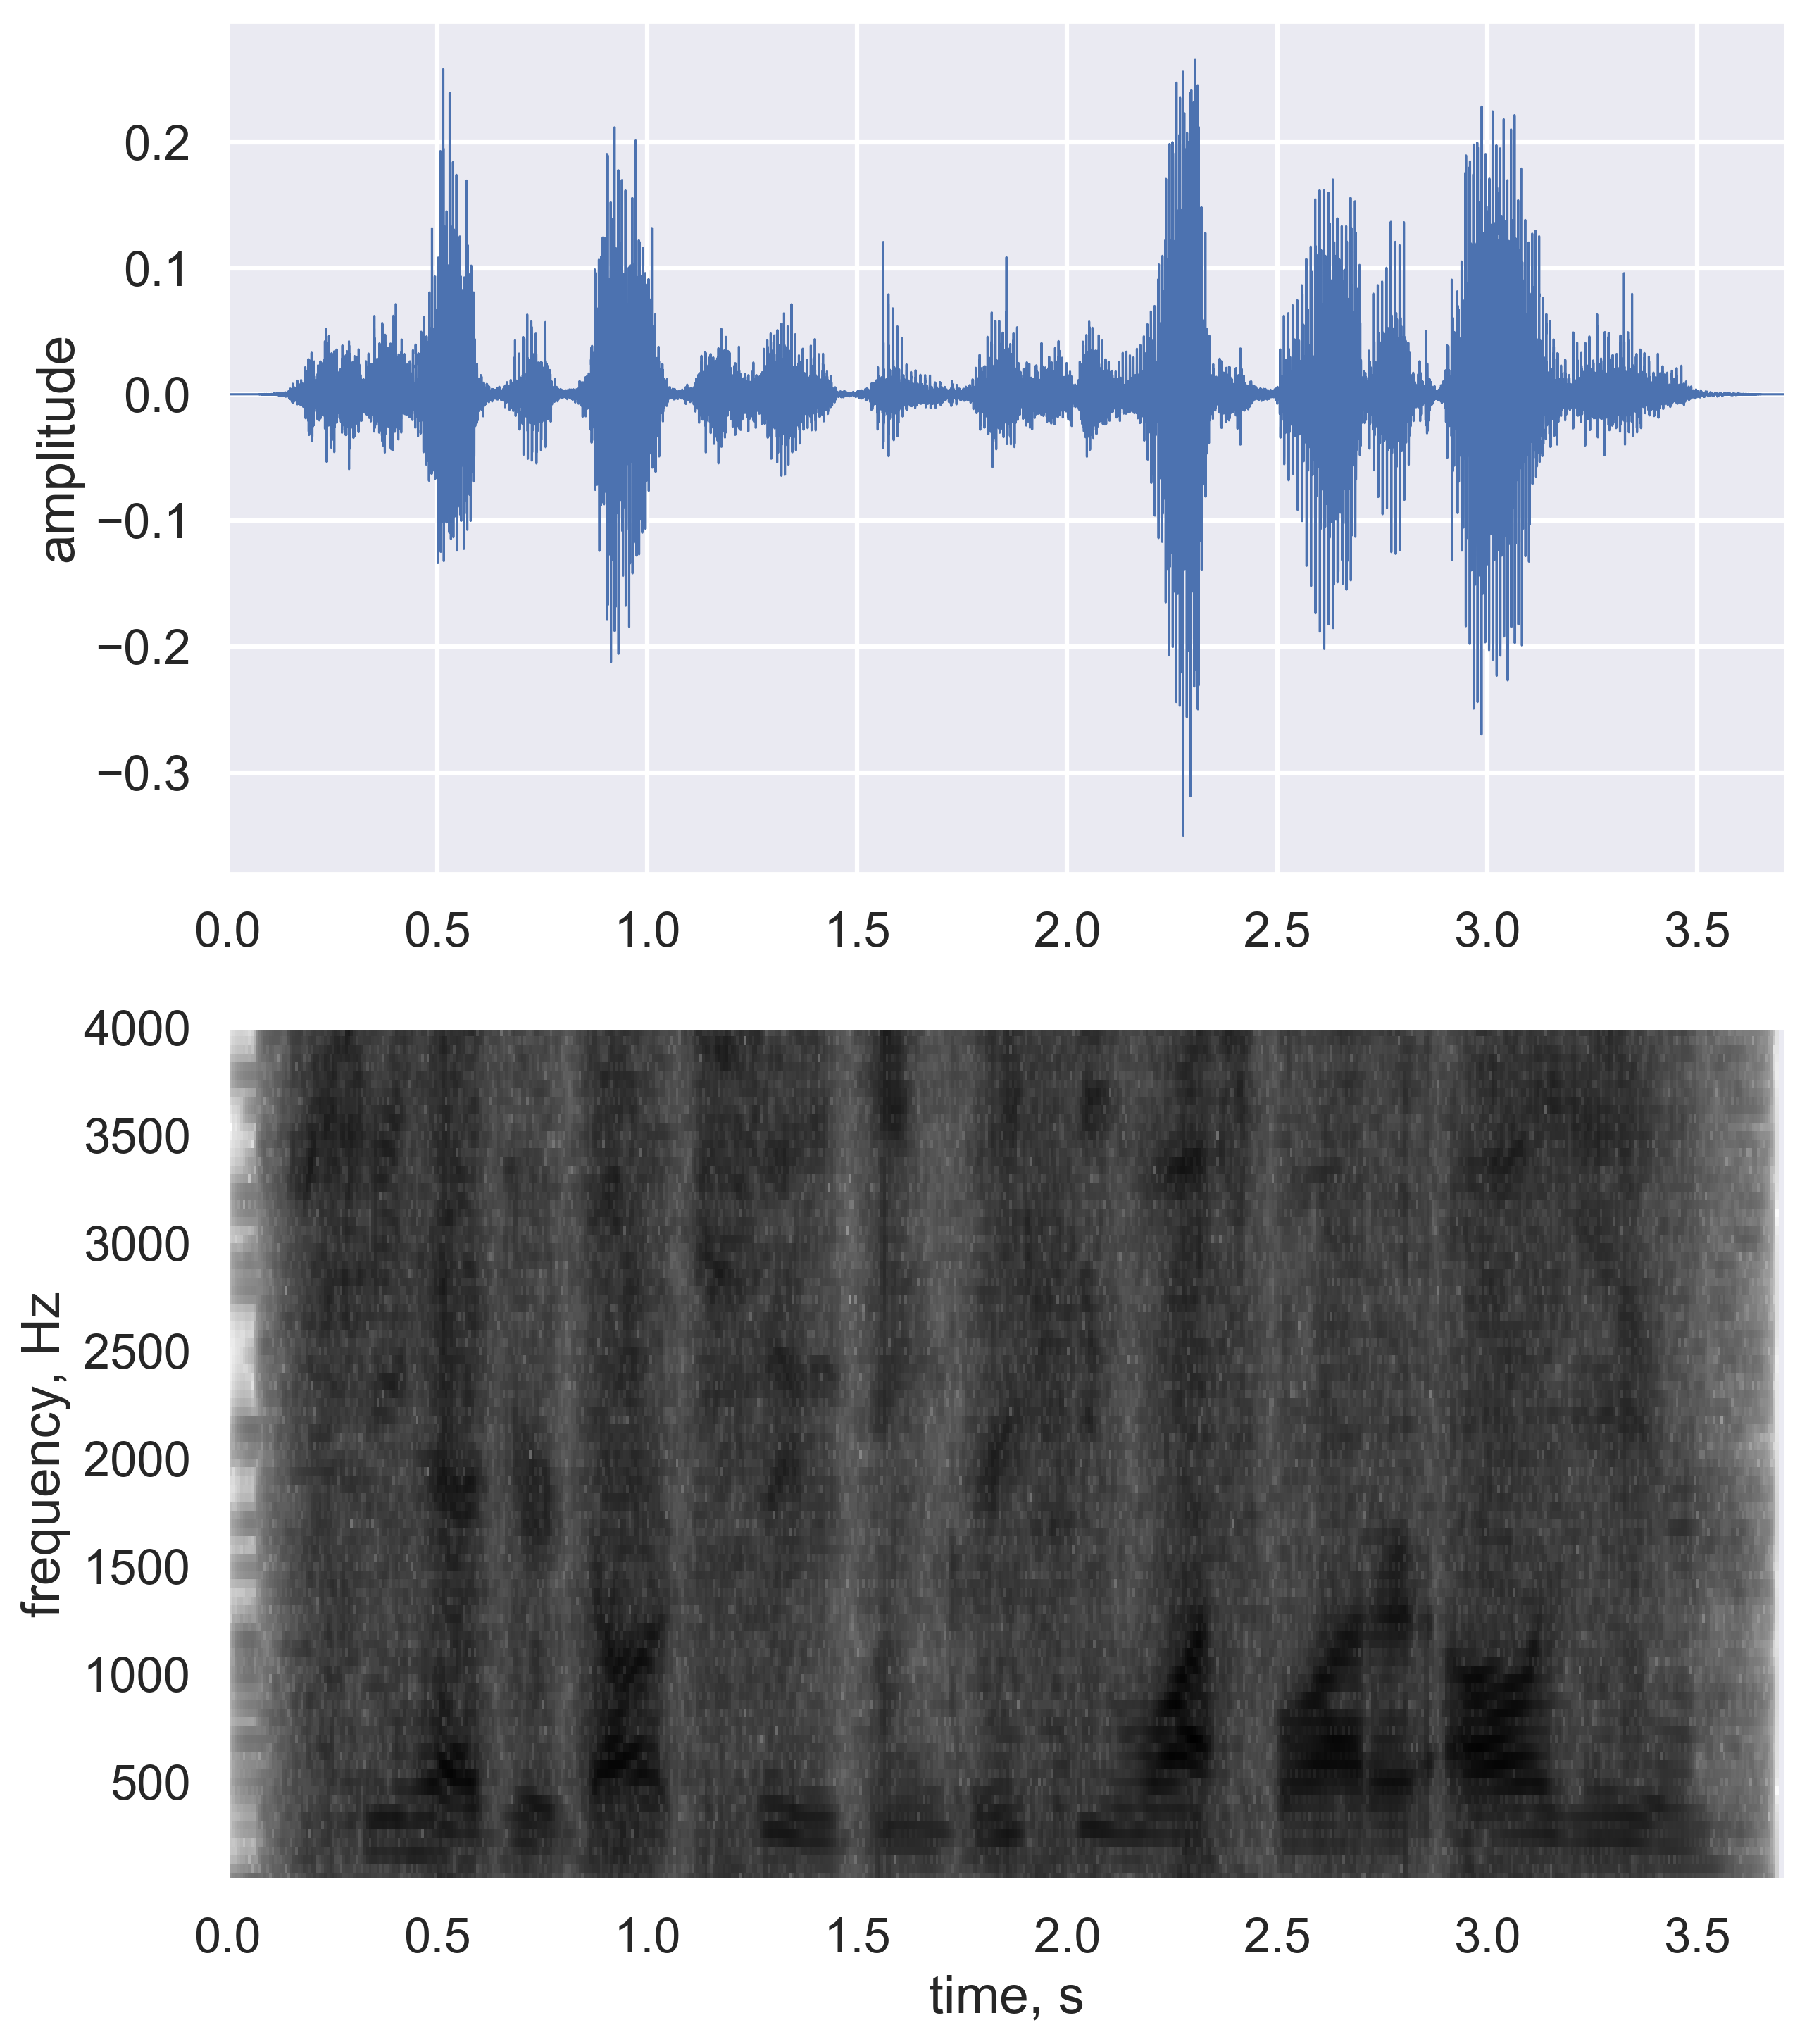
\includegraphics[width=\textwidth]{speech_recover.png}
		\caption{Recovered}
		\label{fig:speech-recovered}
	\end{subfigure}
	\caption{Test speech signal in the time domain (top row) and modulation domain (bottom row).}
	\label{fig:speech}
\end{figure}

\subsection{Processing}
\label{ssec:audio-speech-process}
I compressively sampled the signal with a compression ratio of 40\%, using 1024 frames and 75\% frame overlap. Following the results from Sec.~\ref{sec:audio-algorithms}, I used the LASSO algorithm for reconstruction, once again obtaining the optimal regularization parameter $\alpha$ by 5-fold cross validation.

\subsection{Reconstruction evaluation}
\label{ssec:audio-speech-metric}
The reconstruction quality was quantified using the International Telecommunication Standardization Sector (ITU-T) recommendation P.862 \cite{pesq}, otherwise known as the Perceptual Evaluation of Speech Quality (PESQ). This metric is a full-reference, perceptually intuitive scoring system which models the now-obsolete mean opinion scores (MOS). This algorithm performs a series of standardized tests modeled after qualitative metrics, analyzes and compares the original and reconstructed signals, and returns a value from 1.0 (bad) to 5.0 (perfect). Because real reconstructed signals are rarely exactly the same as the original, the PESQ values are usually thresholded up to 4.5 (excellent). PESQ values of 3.0 and above indicate acceptable quality.

For a more quantitative test, I also used the average segmental signal-to-noise ratio (SNR\textsubscript{seg}) \cite{Loizou2013}, defined as

\begin{equation}
	\label{eq:snrseg}
	\mathrm{SNR_{seg}} = \frac{10}{B} \sum_{b=0}^{B-1} \log_{10} \frac{\sum_{i = Nb}^{Nb + N - 1} x_i^2}{\sum_{i = Nb}^{Nb + N - 1} (x_i - \hat{x}_i)^2}
\end{equation}

\noindent where $N$ is the frame length, $B$ is the number of frames, $x_i$ are the original signal samples, and $\hat{x}_i$ are the reconstructed signal samples.

Figure~\ref{fig:speech-recovered} shows the reconstructed signal. Qualitative comparison in the time domain shows that the original and reconstructed waveforms are structurally similar. In the modulation domain, the dynamic range of the latter seems to have diminished, but the dominant frequencies can still be observed. Evaluation of the PESQ and SNR$_\mathrm{seg}$ yields values of 2.50 and 0.07, respectively. At face value, I can immediately tell from the PESQ that the reconstructed signal quality is slightly below average; listening to the reconstructed recording reveals a noticeable level of noise in the background. However, the same distinction cannot be made for the SNR$_\mathrm{seg}$ since its bounds are not well-defined.

\subsection{Error space analysis}
\label{ssec:audio-speech-error}
Using the same test signal, I generated the error space maps by compressively sampling the signal and evaluating the metrics for varying compression $\textrm{ratios} \in [0.1, 0.9]$ in increments of 0.1, and varying number of $\textrm{frames} \in \{128, 256, 512, 1024\}$, while keeping the frame overlap constant at 75\%. Figure~\ref{fig:speech-error} shows the PESQ and SNR$_\mathrm{seg}$ maps. The former exhibits a sensitivity to the compression ratio, and achieves the acceptable threshold of 3.0 at around 60\% compression. The latter shows sensitivity towards the number of frames (as it is an \textit{average} metric) with some additional degradation below 40\% compression ratio. It achieves a maximum value of 0.08 at around 1024 frames.

\begin{figure}[htb]
	\centering
	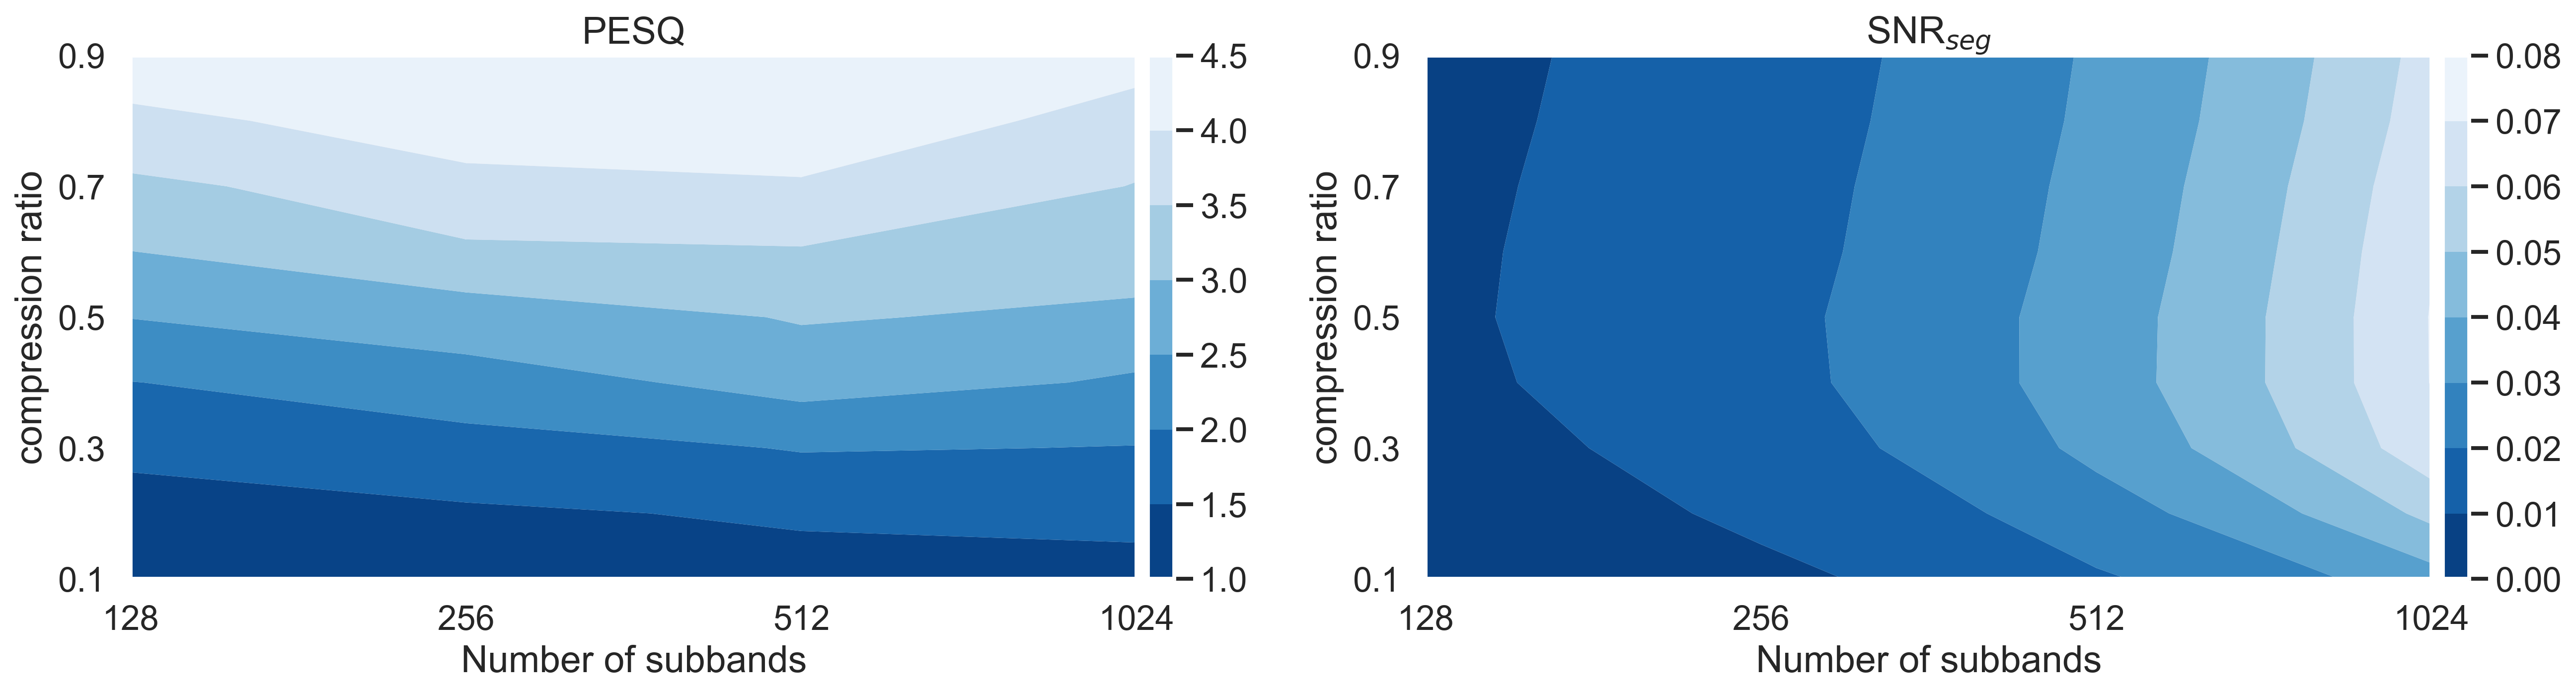
\includegraphics[width=\textwidth]{speech_metrics.png}
	\caption{Evaluation of PESQ and SNR$_\mathrm{seg}$ error space maps as a function of compression ratio and number of subbands, using the same speech recording in Fig.~\ref{fig:speech}}
	\label{fig:speech-error}
\end{figure}
\chapter{Conclusions}
\label{chap:conc}

\appendix
\chapter{Codes and Implementations}
\label{appendix:codes}

\singlespacing
\lstset{
	basicstyle=\footnotesize\ttfamily,
	commentstyle=\itshape\color{green!50!black},
	keywordstyle=\bfseries\color{Purple},
	stringstyle=\color{red!70!black},
	numberstyle=\footnotesize\ttfamily,
	numbersep=15pt,
	tabsize=4,
	frame=lines,
	language=Python,
	numbers=left,
	label={code:1d-test},
	caption={Code for compressive sensing of 1D test sinusoids.}
}
\lstset{morekeywords={as, True, False}}
\begin{lstlisting}
import numpy as np
import numpy.random as rand
import scipy.fftpack as fft

# load recording
signal = np.loadtxt("piano.txt").astype("float32")

# define parameters
samprate = 44.1e3
duration = 1/8
N = int(duration*samprate)
M = 300
t = np.linspace(0, duration, N)

# extract short portion of recording
sig_start = 40000
x = signal[sig_start:sig_start + N]

# simulate compressive measurements
yi = rand.randint(0, N, M)
yi = np.sort(yi)
y = x[yi]

# L1 optimization using CVX ECOS
import cvxpy as cvx
xhat_cvx = cvx.Variable(N)
objective = cvx.Minimize(cvx.Norm(xhat_cvx, 1))
constraints = [A*xhat_cvx == y]
prob = cvx.Problem(objective, constraints)
result = prob.solve(verbose=True, solver="ECOS")
x_cvx = np.array(xhat_cvx.value)
x_cvx = np.squeeze(x_cvx)
x_cvx = fft.dct(x_cvx, norm="ortho", axis=0)

# L1-regularized L2 optimization using LASSO
from sklearn.linear_model import Lasso, LassoCV
lasso = LassoCV(cv=10, random_state=0, verbose=True, n_jobs=-1)
lasso.fit(A, y)
x_lasso = fft.idct(lasso.coef_)
\end{lstlisting}

\lstset{
	label={code:random},
	caption={Code for generating different random distributions.}
}
\begin{lstlisting}
from sklearn.metrics import mean_squared_error
# define parameters
samprate = 44.1e3
duration = 1/32
N = int(duration*samprate)
M = np.arange(50, N+1, 50)
t = np.linspace(0, duration, N)

# define normalization function
def normalize(x):
	x = x.astype(float)
	x /= x.max()
	return x

# evaluate errors
y_uniform_errs = []
for m in M:
	trial_err = []
	for i in range(10):
		yi = rand.uniform(0, N, m)
		yi = np.sort(yi)
		y_uniform = signal[yi]
		d = np.identity(N)
		d = fft.dct(d)
		A = d[yi]
		lasso = Lasso(alpha=0.1)
		lasso.fit(A, y_uniform)
		xhat_uniform = fft.idct(lasso.coef_)
		mse = mean_squared_error(normalize(signal), normalize(xhat_uniform))
		trial_err.append(mse)
	y_uniform_errs.append(trial_err)
\end{lstlisting}

\bibliographystyle{spp-bst}
\bibliography{library,thesis}

\end{document}